% !TeX program = xelatex
% 保留编辑器当前文件为工程主入口；正文、表格、图片在paper/中。
\documentclass[UTF8,a4paper,zihao=-4,fontset=fandol]{ctexart}
\usepackage[margin=25mm,top=23mm,bottom=24mm]{geometry}
\usepackage{amsmath,amssymb}
\usepackage{graphicx,booktabs,array,longtable}
\newcolumntype{L}[1]{>{\raggedright\arraybackslash}p{#1}}
\usepackage{caption}
\usepackage[section]{placeins}
\usepackage{xurl}
\usepackage[unicode,hidelinks]{hyperref}
\hypersetup{pdftitle={基于体检指标与异质模型融合的血糖回归预测及预处理对照研究}}
\ctexset{section={format=\Large\bfseries},subsection={format=\large\bfseries},subsubsection={format=\normalsize\bfseries}}
\captionsetup{font=small,labelfont=bf,labelsep=quad}
\linespread{1.20}
\setlength{\parindent}{2em}
\setlength{\emergencystretch}{2em}
\setlength{\aboverulesep}{0.5ex}
\setlength{\belowrulesep}{0.5ex}
\renewcommand{\arraystretch}{1.18}
\setcounter{topnumber}{3}
\setcounter{bottomnumber}{2}
\setcounter{totalnumber}{5}
\renewcommand{\topfraction}{0.9}
\renewcommand{\bottomfraction}{0.8}
\renewcommand{\textfraction}{0.08}
\renewcommand{\floatpagefraction}{0.7}
\raggedbottom
\pagestyle{plain}
\begin{document}
\begin{center}
{\Large\bfseries 基于体检指标与异质模型融合的\\[0.25em]血糖回归预测及预处理对照研究}
\end{center}

\begin{abstract}
针对利用临床及体检指标预测个体血糖浓度的竞赛任务，本文在保留全部待评价记录的条件下，研究缺失处理、特征构造、模型选择与异质回归模型融合。将原训练集与带标签A集合并，固定划分为4649条训练记录和1993条开发记录；缺失填补、标准化与可选主成分分析均限定在相应训练部分拟合。首先比较六类基准模型，随后依次进行特征分组消融、有限预算联合参数搜索、树与线性模型融合、小型神经网络及其补充融合，利用训练折外预测确定配置与权重。最终方案由优化XGBoost、LightGBM、Ridge和去除乙肝五项的小网络各占25\%组成，其开发集和B集均方误差分别为2.177243和1.234296，相对原XGBoost分别降低约2.31\%和1.47\%。进一步固定十个模型版本的特征、参数和网络轮数，开展标准化与主成分分析的四处理对照。结果表明，本轮两个网络从标准化中获得较低的训练折外误差，额外增加主成分分析未显示稳定收益；仅调整推荐预处理的融合版本在开发集略有改善，在B集略有变差。最终融合对高血糖值仍有低估，B集相对基线的配对误差差异区间跨零。由于开发集和B集均有历史研究使用，结果属于已知数据上的复核，尚不能证明未来样本上的稳定优势。
\end{abstract}
\noindent\textbf{关键词：}血糖预测；体检数据；缺失值处理；模型融合；预处理对照

\section{问题重述}\label{sec:problem}

\subsection{竞赛背景与预测任务}
天池精准医疗大赛初赛以临床数据和体检指标为输入，以个体血糖值为预测目标。尽管赛事总体背景涉及糖尿病及遗传风险，本文所用数据和模型均对应初赛的连续血糖回归任务。研究不包含遗传变量建模，也不将血糖回归结果转换为未经验证的糖尿病分类或诊断结论。

数据按记录行组织，每行表示一个个体，首列为ID。训练表包含42列，最后一列为目标血糖值；本地A、B特征表各包含41列，不含目标列。字段涉及性别、年龄、体检日期及多类检验指标，部分检验值缺失。研究需要在有限样本及不完整输入条件下，为每条待预测记录给出连续数值。

\subsection{输出与评价要求}
设评价集合为$E$，样本数为$n_E$，第$i$条记录的真实值与预测值分别为$y_i$和$\hat y_i$。竞赛以均方误差评价预测结果：
\begin{equation}
\operatorname{MSE}_E=\frac{1}{n_E}\sum_{i\in E}(y_i-\hat y_i)^2.
\label{eq:mse}
\end{equation}
误差越低，说明该评价集合上的平方损失越小。初赛提交要求预测值保留小数点后三位。本文报告的是既有实验基于未舍入预测计算的指标，三位小数属于最终提交的数值格式要求，不能将两种计算口径混称为同一提交成绩。

题目还提出高精度、高效和解释性要求。本文以同协议预测误差考察精度，以实际搜索预算说明计算范围，并通过线性探索、特征消融、融合组成与误差诊断分析模型行为。现有研究未包含统一硬件下的效率比较或最终融合的个体预测解释验证，因此相关讨论限定于已有证据。

\section{问题分析}\label{sec:analysis}

\subsection{缺失值与样本覆盖}
不同检验项目的缺失程度存在较大差异，且若干项目具有相同或接近的缺失模式。直接删除缺失比例较高的记录，会同时改变训练样本量和研究人群；若在评价时删除难以预测的记录，还会使所得误差偏离完整预测任务。因而，当前主协议保留全部训练、开发和B集记录，采用折内中位数填补与缺失指示，或采用模型原生缺失处理。

缺失模式可能包含检测安排或样本批次的信息，但现有材料不足以确定其形成机制。本文将缺失计数作为可验证的预测特征，不预设缺失为完全随机，也不赋予其未经证实的医学含义。

\subsection{相关性、量纲与特征表示}
多个体检指标存在统计相关，线性模型可能出现系数不稳定。正则化能够在保留相关变量的同时限制系数规模；标准化则改变不同量纲输入在模型训练中的相对尺度。PCA通过输入方差构造低维表示，其方差保留比例并不直接衡量血糖预测信息。因此，是否缩放、删列或压缩输入，应以训练内部预测比较为依据，而非仅依据相关图或累计方差曲线。

\subsection{非线性关系与误差互补}
线性模型为关联分析和预测提供基准，树模型能够表达轴向阈值与非线性交互，前馈网络则提供另一类连续函数表示。由于不同模型的归纳偏好和特征处理不同，其误差未必完全重合。融合是否有效，取决于同一批记录上的联合误差，而不能只由单模型排名决定。本文使用训练折外预测比较有限个融合配置，避免以模型对自身训练记录的拟合预测选择权重。

\subsection{评价边界与尾部误差}
MSE对较大误差更敏感，少量高目标值记录可能贡献较多平方损失。仅比较总体指标不足以说明误差分布，需要结合分箱诊断与配对误差差异分析。另一方面，表示选择、参数搜索和权重筛选均会引入选择偏差，重复使用开发或B集也会限制结论的外推。因此，本文分别报告训练内部选择、配置冻结后的已知集合复核及其条件不确定性。

\section{模型假设与符号说明}\label{sec:assumptions}

\subsection{建模设定}
本文将提供的血糖标签作为监督目标，将同名体检字段作为预测时可取得的输入。逐行特征构造只使用该记录的输入，不使用真实血糖、ID或日期；需要从数据估计的变换统计量仅在相应拟合行上计算。当前主协议保留未知性别、原始连续年龄、缺失记录和极端检验记录。

上述设定不等于已验证输入测量无误或样本独立同分布。现有材料没有提供患者身份键、完整计量单位及采样条件，本文不额外假设不存在同人多次体检，不指定空腹状态，也不为使用平方损失而假设真实血糖或残差服从正态分布。行重采样区间的条件解释在第\ref{sec:evaluation}节讨论。

\subsection{主要符号}
表\ref{tab:symbols}列出全文主要符号。各模型特有参数在首次使用时进一步定义。未提供的血糖与检验单位不作推定，数值沿用原数据尺度。
\begin{table}[htbp]
\small
\setlength{\tabcolsep}{5pt}
\centering
\caption{主要符号及含义}
\label{tab:symbols}
\begin{tabular}{L{0.27\linewidth}L{0.65\linewidth}}
\toprule
符号 & 定义 \\
\midrule
$\mathcal D_T,\mathcal D_V,\mathcal D_B$ & 当前训练、开发与B集合，分别4649、1993、1000行 \\
$F,n_F$ & 某次实际拟合行集合及其样本数；包括折内、内部子集或完整拟合集 \\
$x_i,y_i,\hat y_i$ & 第i条记录的输入、真实血糖与预测血糖 \\
$n_T,p$ & 训练行数及当前表示的输入列数；p随特征与变换改变 \\
$\Phi_F,\phi_i$ & 只在F拟合的编码/预处理组合及其输出向量 \\
$m_{ij},q_j(F),J_F$ & 缺失指示、拟合列中位数及拟合时出现缺失的列集合 \\
$u_i,z_i,t_i$ & 填补并加指示后的向量、标准化向量、PCA得分 \\
$\xi_i,\zeta_i$ & 40维训练探索填补向量及其标准化表示，不加自动缺失指示 \\
$I_{s,k},\mathcal E_s(c)$ & 种子s的第k验证折及候选c的合并OOF损失 \\
$\alpha_R,\alpha_L$ & Ridge与Lasso惩罚系数，分别100与0.05 \\
$\eta,\lambda_X,a_X,\gamma_X$ & 提升学习率、XGB叶权L2/L1及叶数惩罚，按模型参数确定 \\
$\pi_m,\Delta_E,Q_g$ & 外层融合权重、候选减参考的MSE差、分箱平方误差贡献 \\
\bottomrule
\end{tabular}
\end{table}


\section{数据预处理与探索性分析}\label{sec:data}

\subsection{数据组织与验证划分}
原训练集包含5642条带标签记录，A、B特征表各包含1000条记录。A答案按有表头读取，B答案按无表头读取，并按文件原有行顺序与特征表匹配。三类特征表的ID互不重复；由于标签文件未含ID，该核对不能独立证明文件提供时的标签排序来源。

当前主协议将原训练集与带标签A集合并为6642条，以随机种子23按70/30划分，得到4649条训练记录和1993条开发记录。开发记录由原训练集1685条与A集308条组成，并非独立的纯A集。表\ref{tab:protocol}区分训练选型、开发评分和B评分的样本范围。
该协议利用研究阶段已取得的A集标签，用于现有数据上的扩展训练与复核，不等同于初赛仅提供原始训练标签时的在线提交协议。仅使用原训练集拟合的历史H2结果在附录\ref{app:history}中单列。
\begin{table}[htbp]
\small
\setlength{\tabcolsep}{5pt}
\centering
\caption{当前主协议的样本与拟合范围}
\label{tab:protocol}
\begin{tabular}{L{0.13\linewidth}L{0.13\linewidth}L{0.12\linewidth}L{0.5\linewidth}}
\toprule
用途 & 拟合/选择行 & 评价行 & 备注 \\
\midrule
训练内部选择 & 4649 & 相应训练验证折 & 原train3957+A692；五折内估计预处理 \\
开发评分 & 4649 & 1993 & 原train1685+A308；不是纯A验证 \\
B集复核 & 6642 & 1000 & 冻结后以train+A全部重拟合；B有历史使用 \\
\bottomrule
\end{tabular}
\end{table}


表示、参数和权重确定后，B评价使用全部6642条重新拟合模型与预处理器，再预测同一1000条B记录。开发和B评价的拟合样本数及目标分布不同，不能由B的绝对MSE较小推断模型性能随之增强。

原训练集日期为2017年9月15日至10月31日，A集为10月10日至10月31日，B集为10月20日至10月31日，日期范围相互重叠。因此，B集不等于严格未来批次。开发集及B集均有历史使用，本文将冻结后评分称为已知集合复核。

\subsection{编码、填补与表示变换}
删除预测输入中的ID与体检日期，性别固定编码为女0、男1，其余取缺失，并增加性别未知指示。39个原始预测字段在增加未知指示后形成40列基础输入；去除乙肝五项后为35列。这些维数均不包含后续自动增加的缺失指示或工程特征。

对某次拟合行集合$F$，令$m_{ij}$表示第$i$行第$j$列是否缺失，$q_j(F)$为该列在$F$中的非缺失中位数。采用填补时，定义
\begin{equation}
\widetilde x_{ij}=\begin{cases}
x_{ij},&m_{ij}=0,\\
q_j(F),&m_{ij}=1,
\end{cases}
\qquad u_i=\bigl(\widetilde x_i,(m_{ij})_{j\in J_F}\bigr),
\label{eq:impute}
\end{equation}
其中$J_F$为拟合行中出现过缺失的列集合。对拟合部分全空的列，按实现保留该列并填为0。显式性别未知指示与填补器的性别缺失指示可能重复，本文保留原实现。所有拟合统计量均来自$F$，评价记录仅应用既定变换。这与将预处理纳入训练管线的原则一致\cite{pitfalls}。

标准化在填补后的向量$u_i$上进行。对第$j$列，令$\mu_j(F)$为拟合均值，$s_j(F)$为以$n_F=|F|$作分母计算的标准差；对于零方差列或实现按浮点误差界判定为近常量的列，$s_j^*(F)$取1，其余取$s_j(F)$，则
\begin{equation}
z_{ij}=\frac{u_{ij}-\mu_j(F)}{s_j^*(F)}.
\label{eq:scale}
\end{equation}
标准化不施于血糖目标；年龄在任何缩放后仍保持浮点数，不转整数。

PCA对实际送入的训练矩阵$A_F$中心化，以其协方差矩阵的特征向量构造投影。设特征值为$\nu_1\ge\cdots\ge\nu_p$，前$r$个方向为$V_r$，则
\begin{equation}
t_i=(A_i-\overline A_F)V_r,\qquad
r=\min\left\{k:\frac{\sum_{j=1}^{k}\nu_j}{\sum_{j=1}^{p}\nu_j}>0.98\right\}.
\label{eq:pca}
\end{equation}
原基准的PCA候选先填补和标准化；第\ref{sec:preprocessing}节另比较不作单位方差缩放的PCA。PCA采用完整奇异值分解，维数由各拟合部分确定\cite{pca}，不把训练探索中的固定成分数施于所有折。

\subsection{分布、缺失与极端值}
4649条训练记录的年龄范围为3至93，均值45.718004。血糖均值5.626855，样本标准差1.474255，范围3.07至38.43；开发集与B集均值分别为5.700527和5.486880。图\ref{fig:age}及图\ref{fig:glucose}展示训练分布。血糖图中的拟合正态曲线仅作参照，较长的右尾并不支持将其视为已通过正态性检验。
\begin{figure}[htbp]
\centering
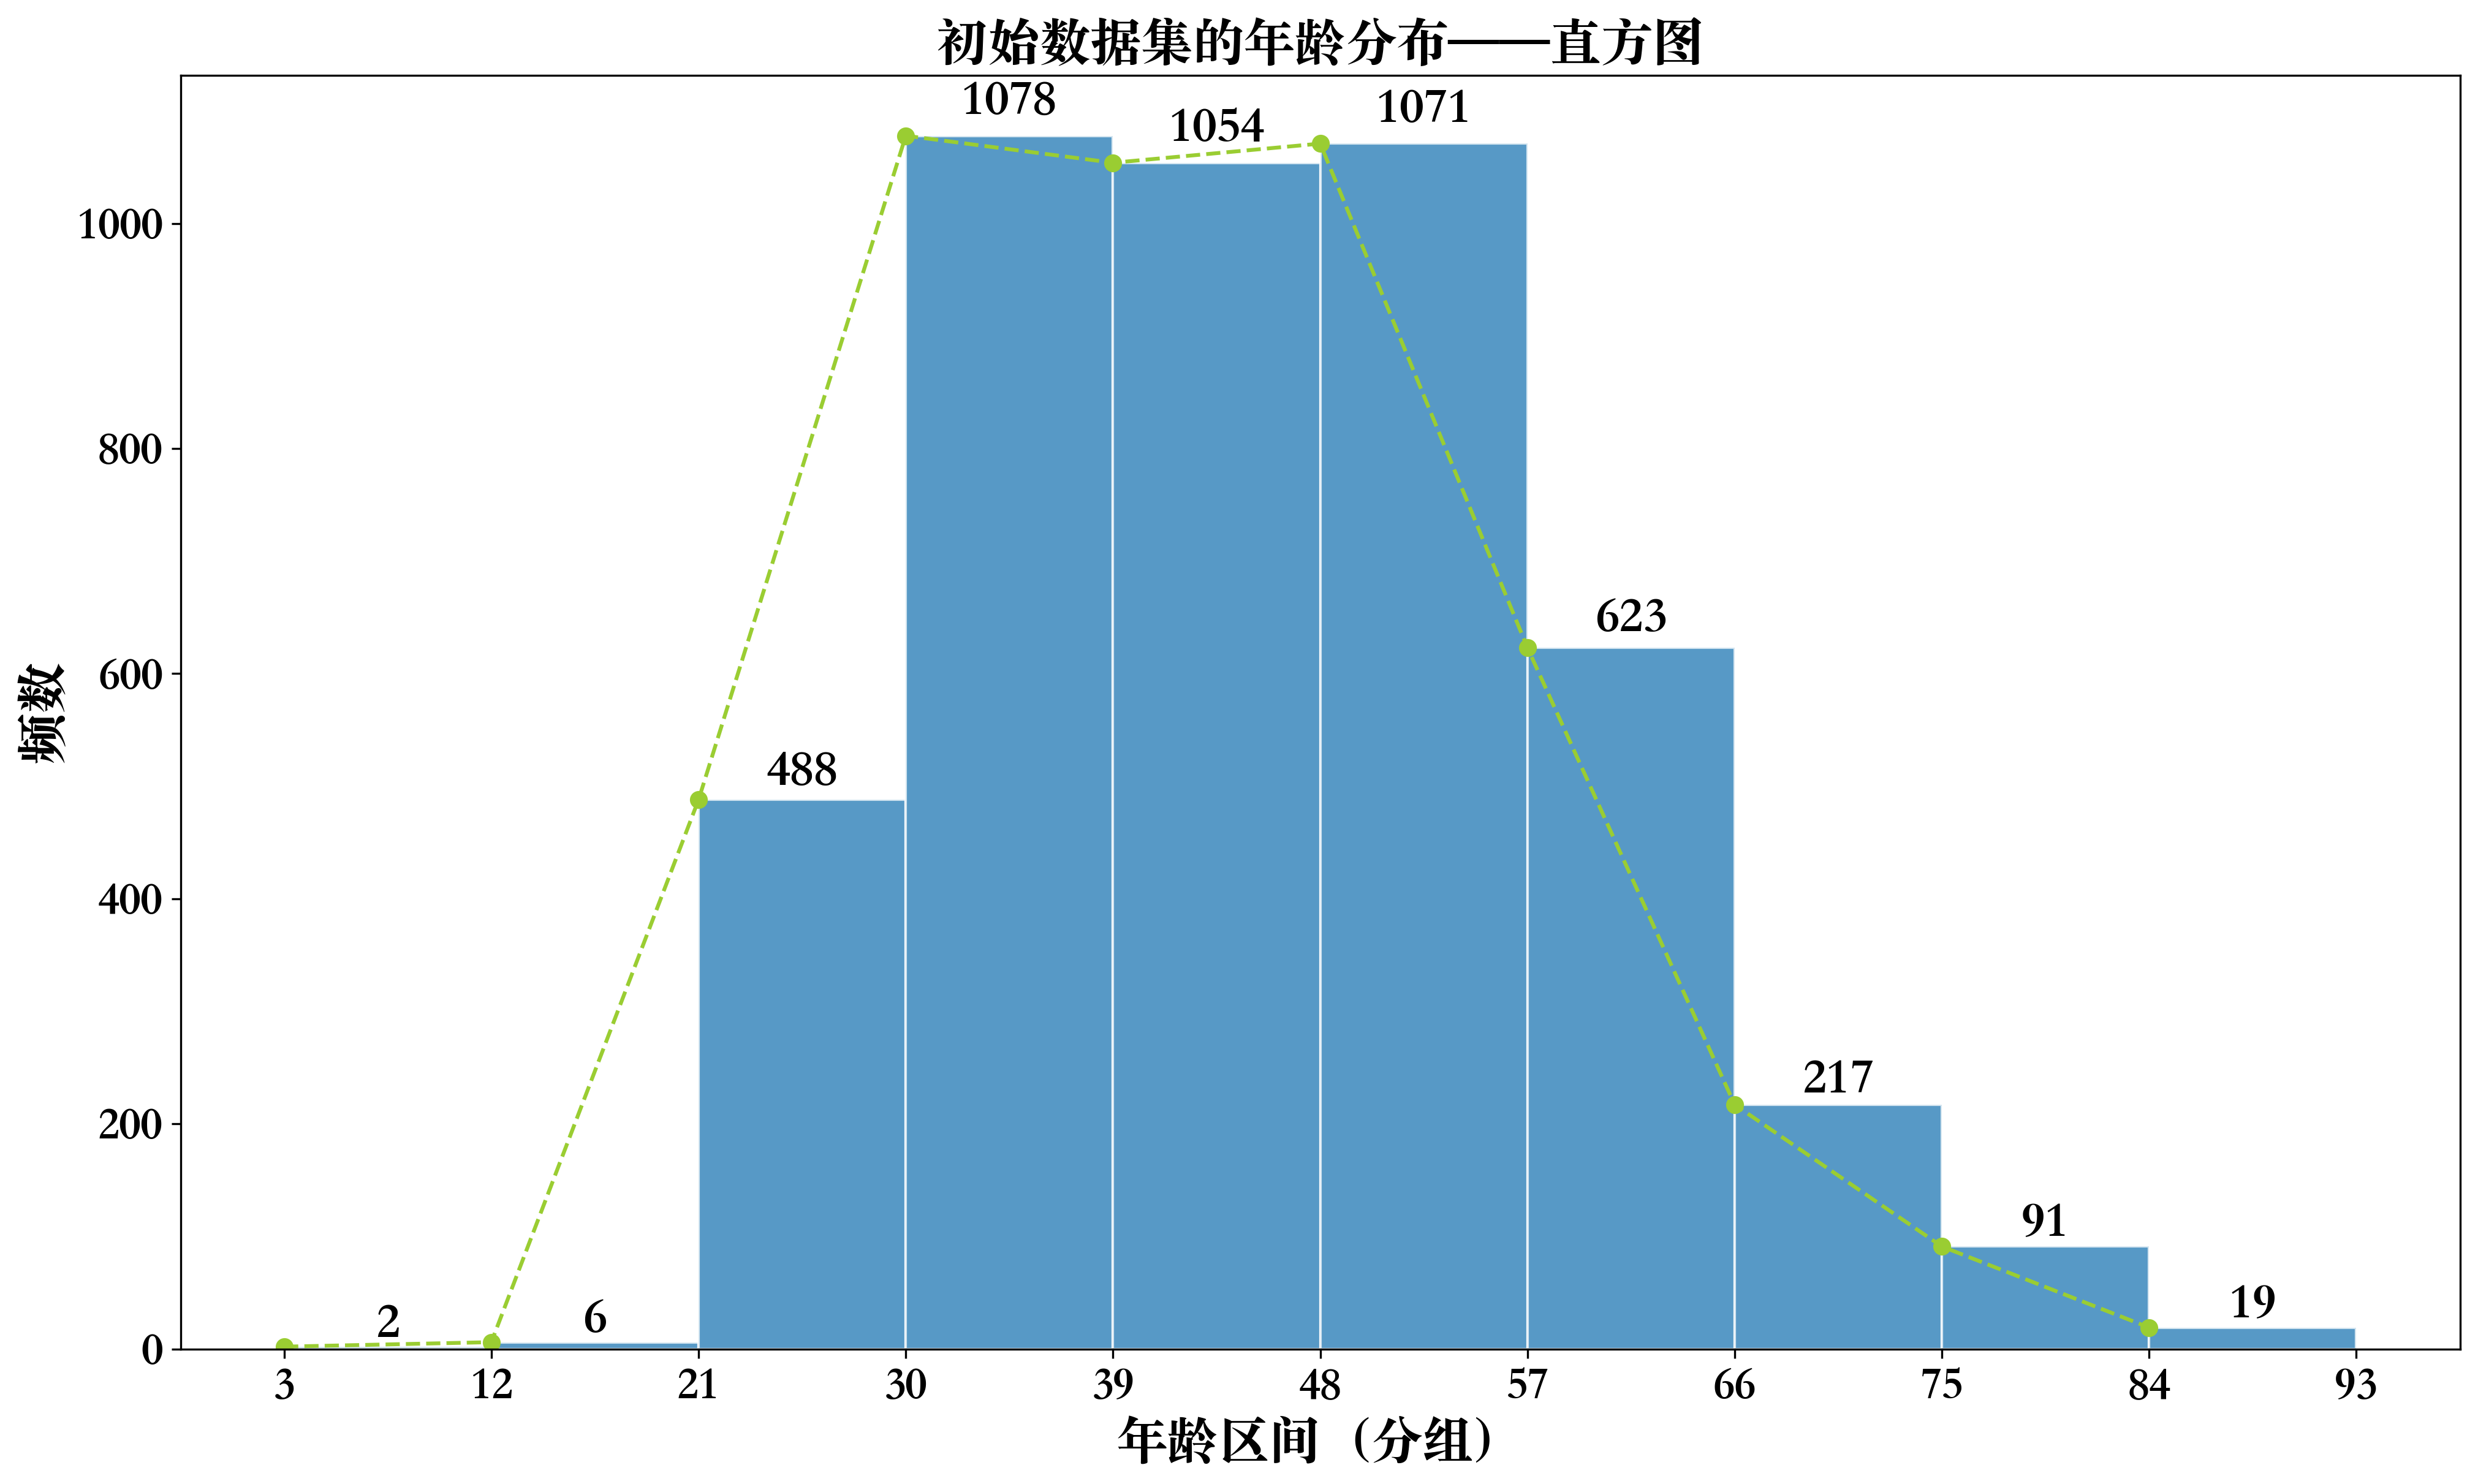
\includegraphics[width=0.94\linewidth,height=0.68\textheight,keepaspectratio]{paper/figures/paper_C007_O03.png}
\caption{4649条训练记录的年龄分布；原图标题中的初始数据指当前训练子集。}
\label{fig:age}
\end{figure}
\begin{figure}[htbp]
\centering
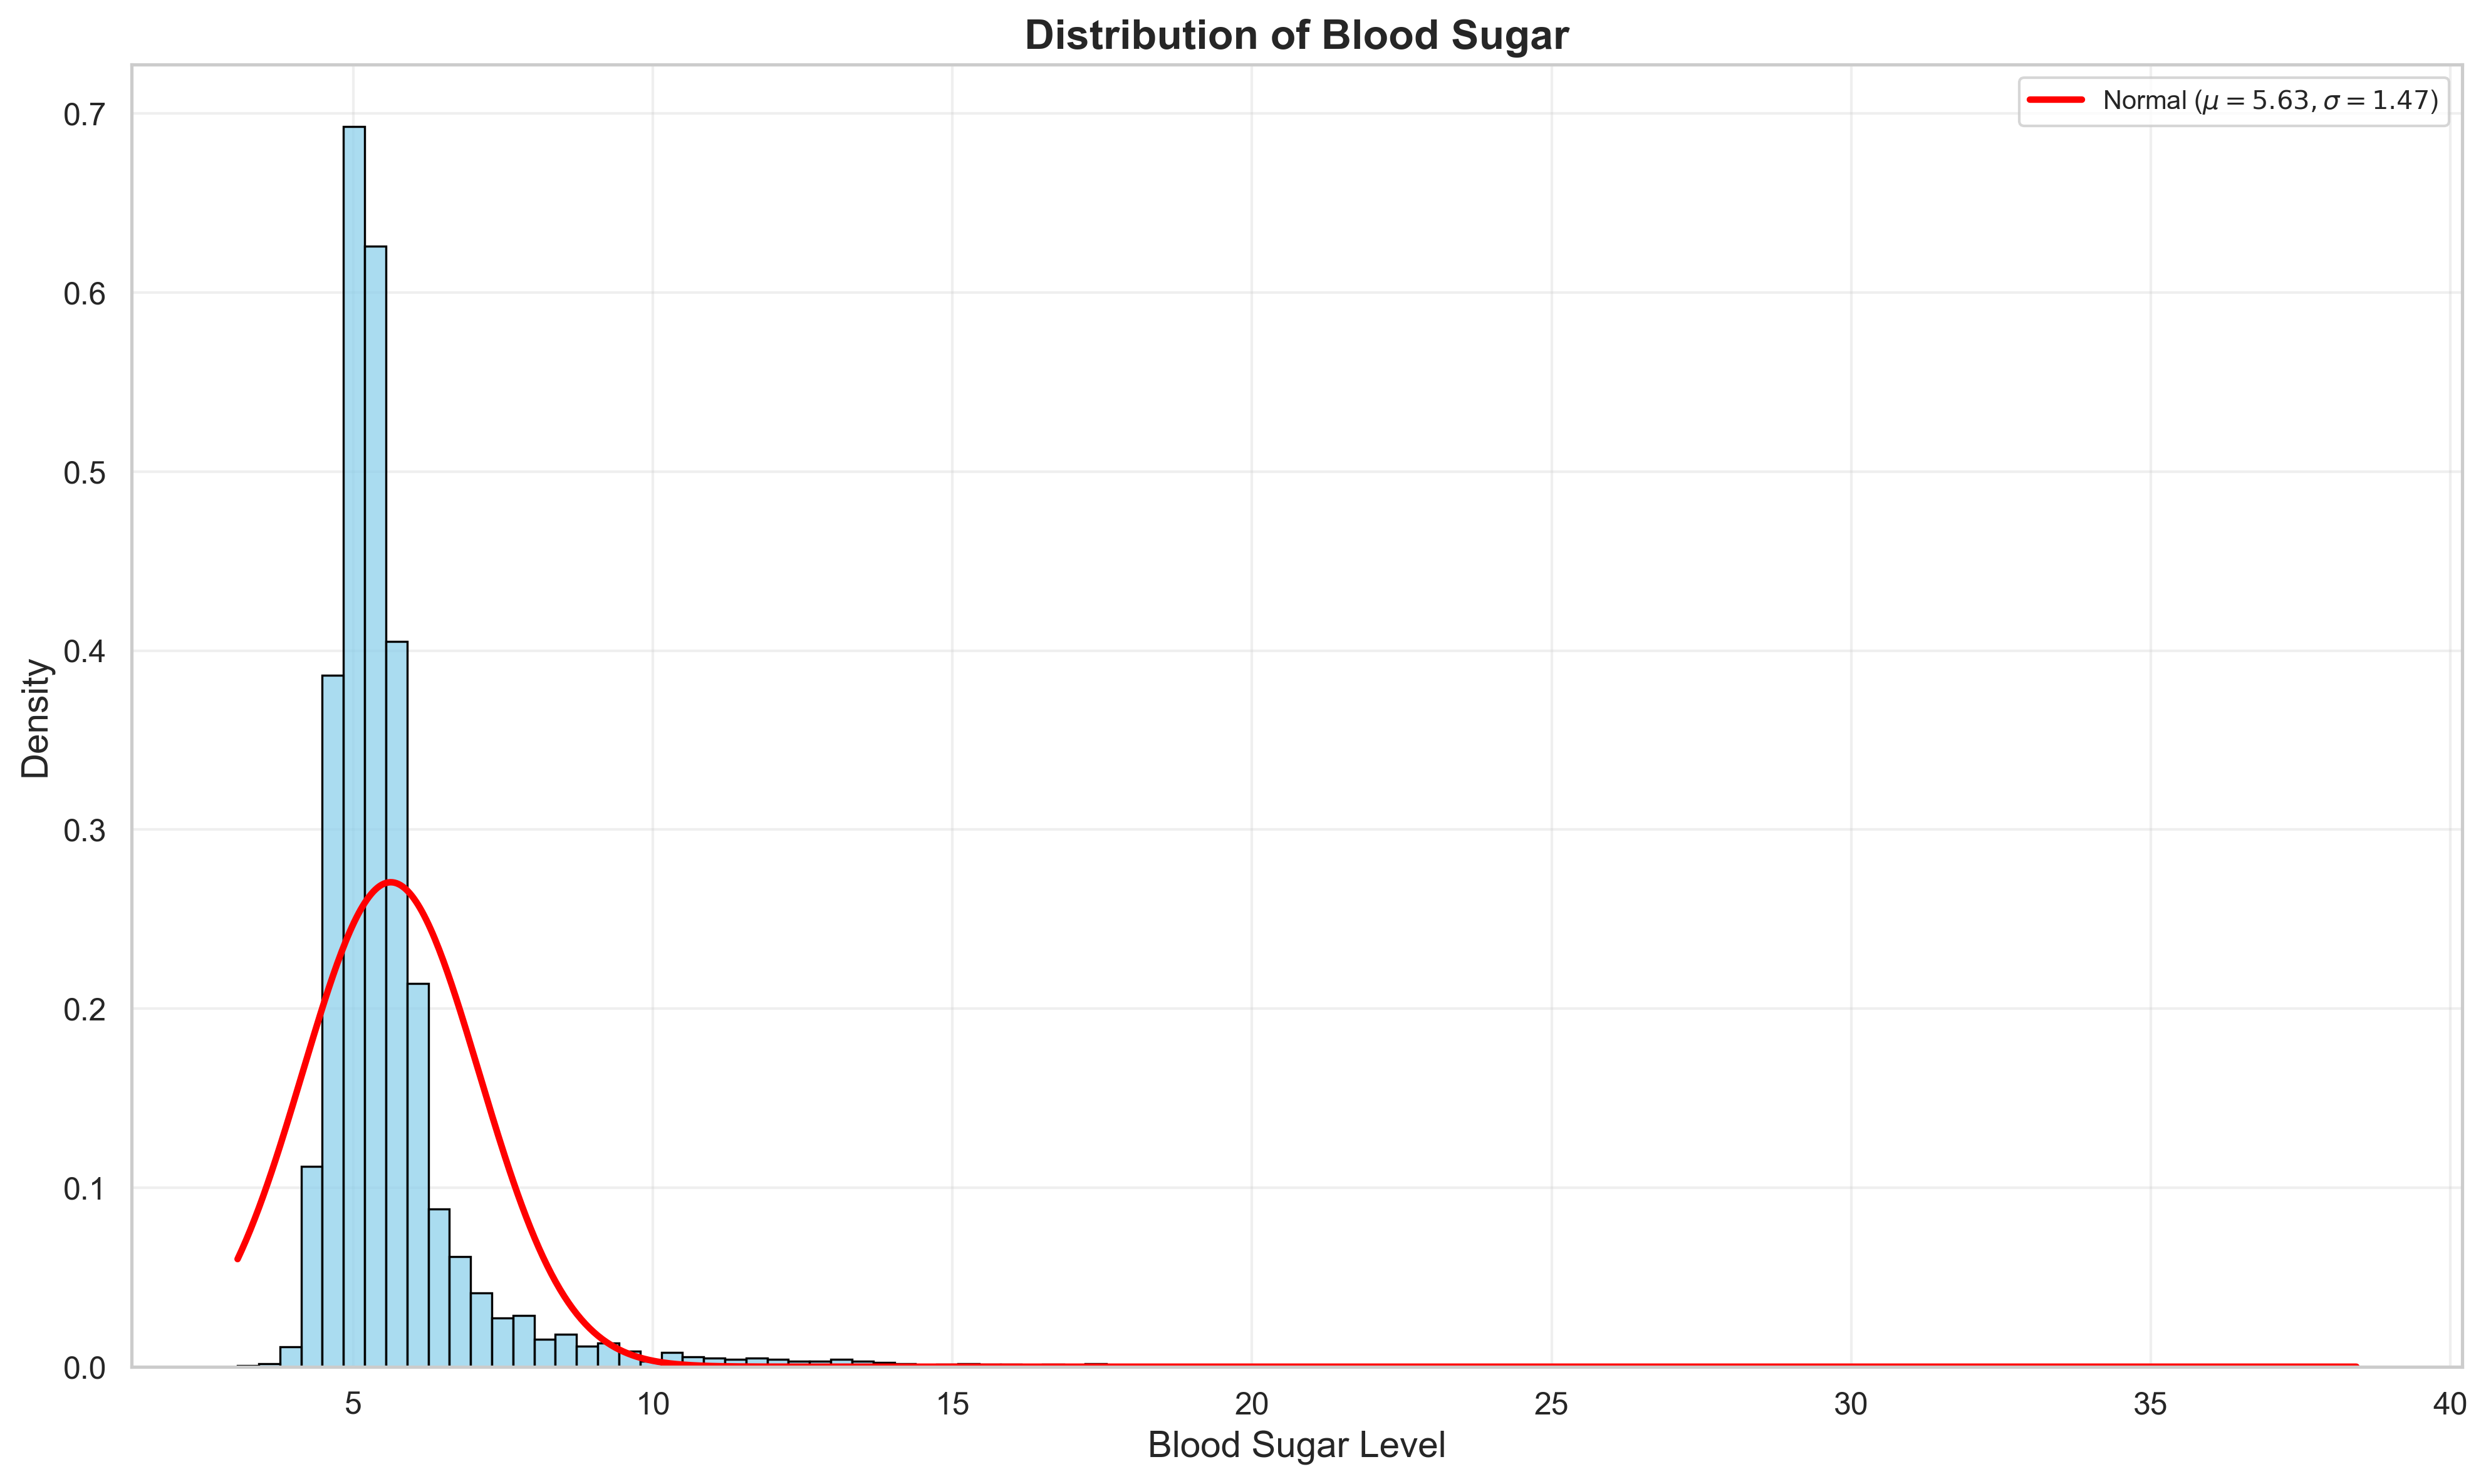
\includegraphics[width=0.94\linewidth,height=0.68\textheight,keepaspectratio]{paper/figures/paper_C009_O01.png}
\caption{4649条训练记录的血糖分布及拟合正态参照曲线；曲线不代表正态性检验结论。}
\label{fig:glucose}
\end{figure}

图\ref{fig:missing}中乙肝五项各缺失76.7047\%，尿素、肌酐、尿酸各缺失23.1233\%，部分肝功能与蛋白指标各缺失20.9507\%。按当前特征口径，1037条训练记录的缺失比例超过20\%，均保留。多个项目的共同缺失及中位数填补会影响探索相关结构，相关热图不能完全解释为生物学联系。
\begin{figure}[htbp]
\centering
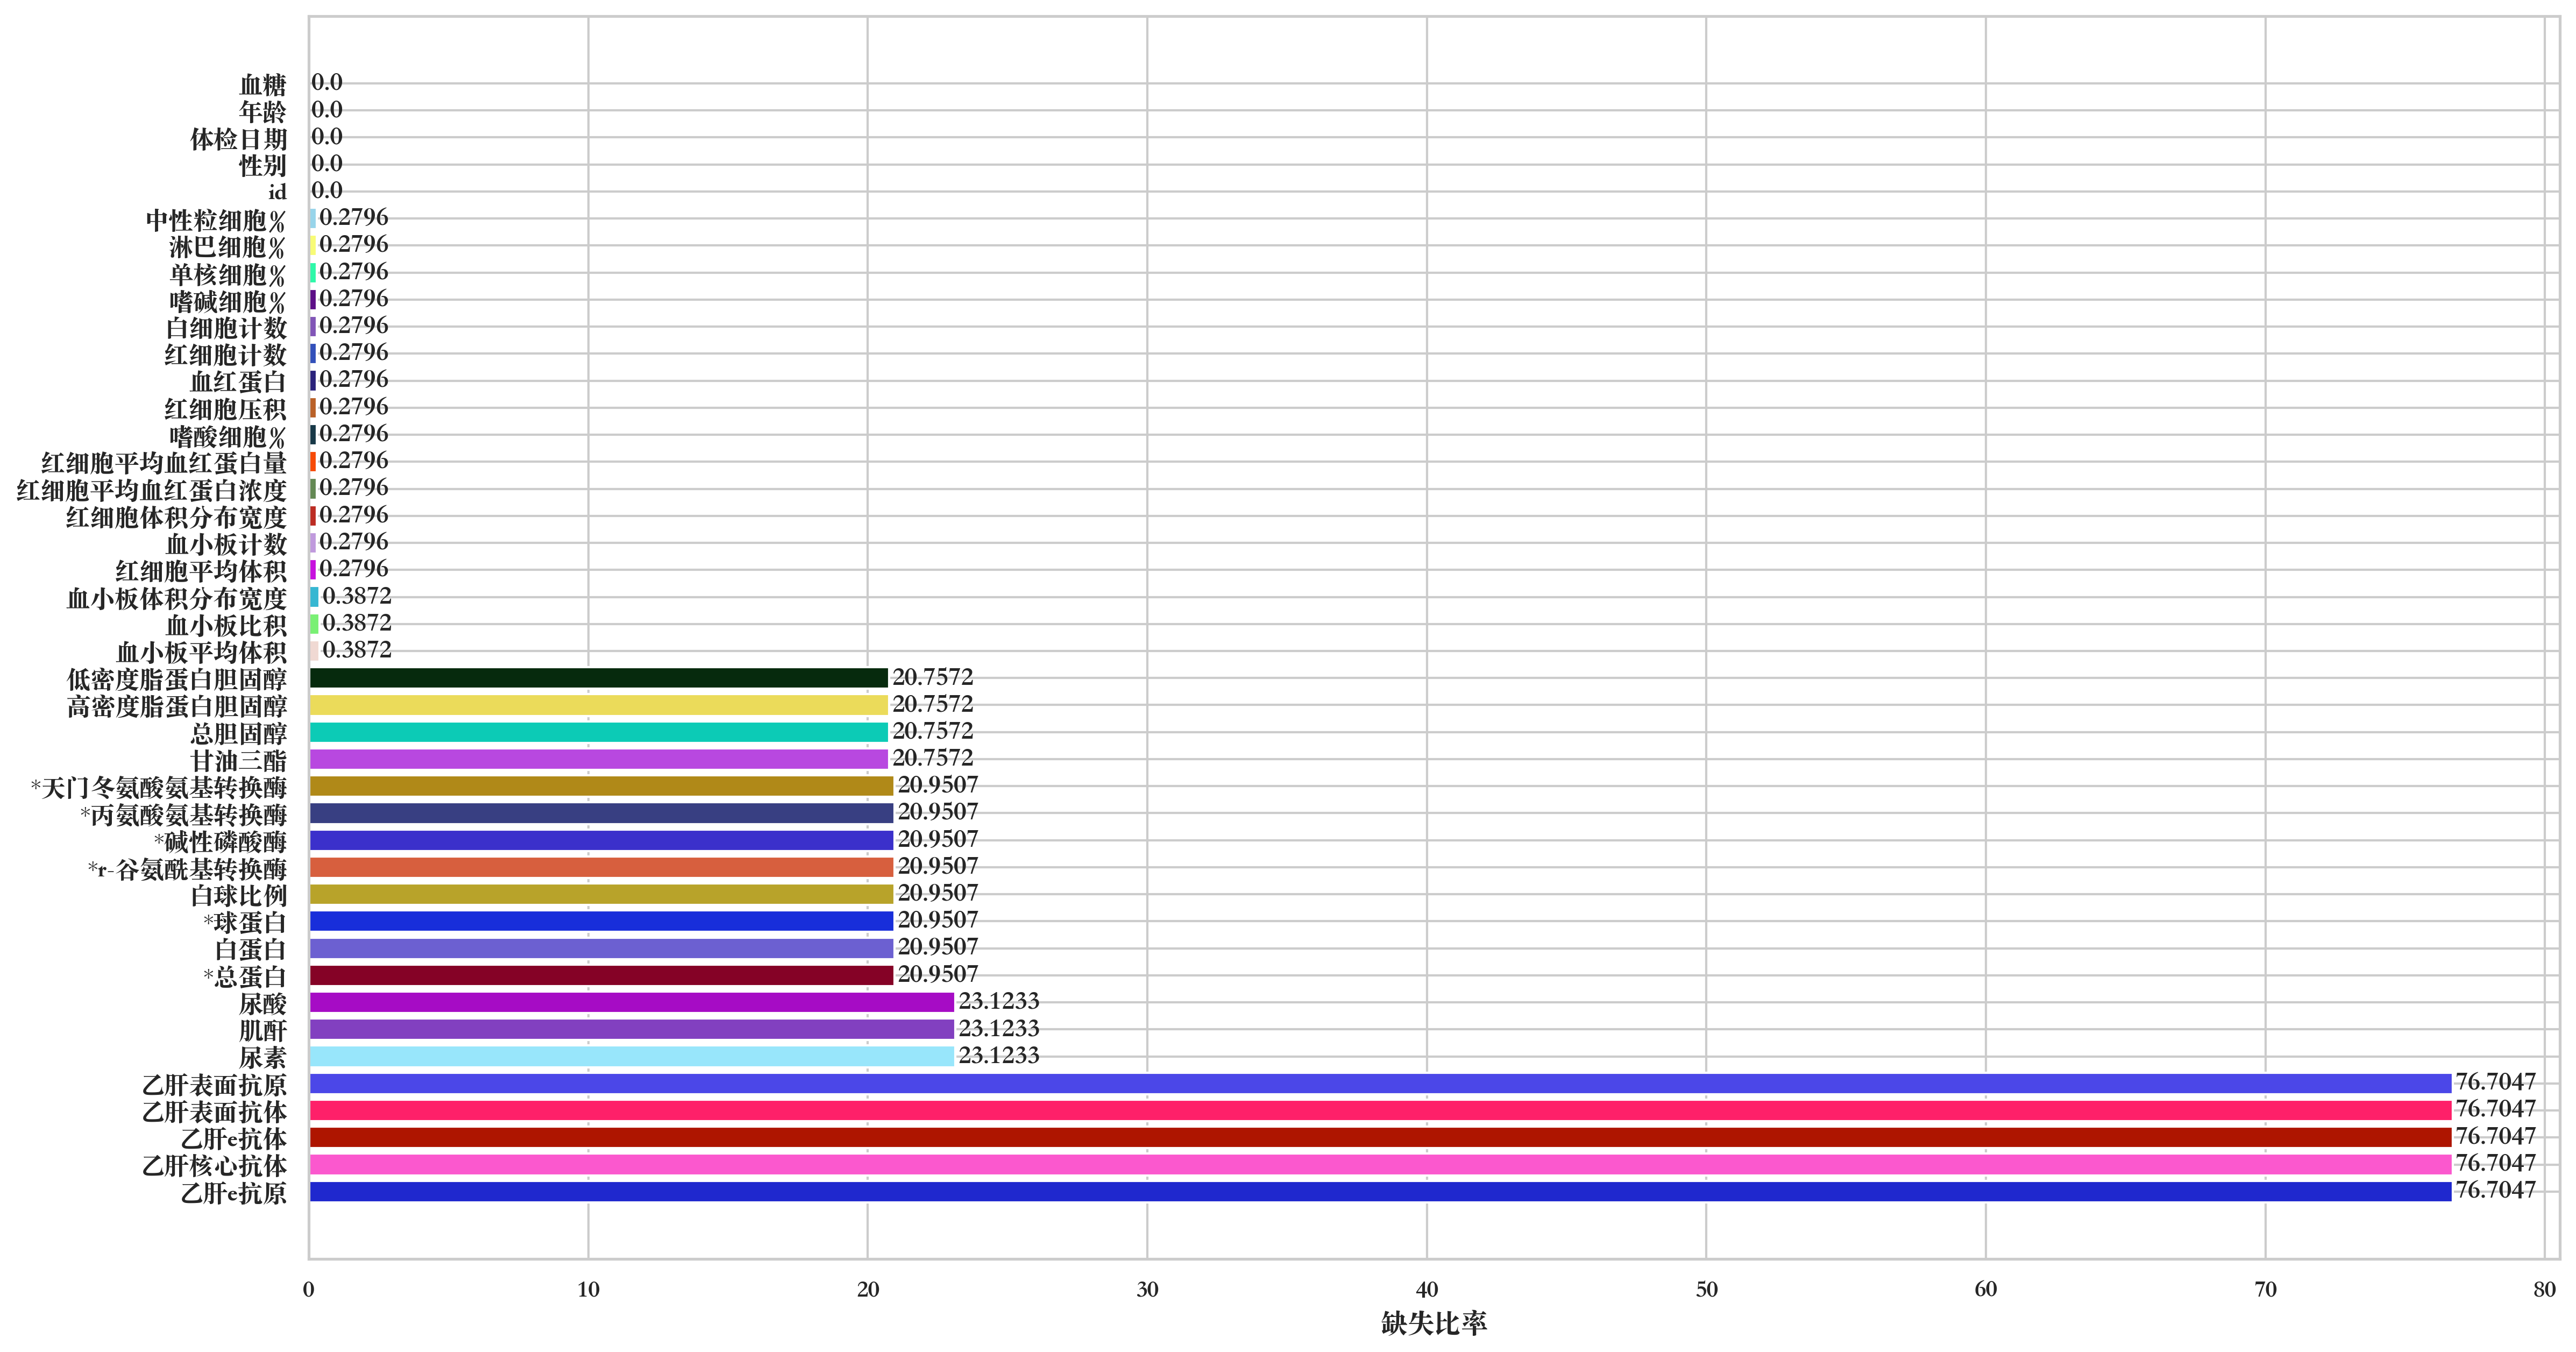
\includegraphics[width=0.94\linewidth,height=0.68\textheight,keepaspectratio]{paper/figures/paper_C012_O02.png}
\caption{4649条训练记录各列缺失比例；原样提取自缺失处理前探索。}
\label{fig:missing}
\end{figure}

探索阶段对既有检验阈值只计数，不删除样本。AST超过200有1条、ALT超过250有2条、GGT超过600有3条、血小板超过600有2条、球蛋白超过60有1条、甘油三酯超过30有2条、肌酐超过175有1条。未发现足以将这些值统一判定为录入错误的依据，故不裁剪输入或血糖目标。

\subsection{线性与降维探索}
令$\xi_i$表示训练探索副本中经中位数填补的40维基础输入，$\zeta_i$为该探索矩阵按训练均值与方差标准化后的向量。采用含截距的普通最小二乘进行拟合诊断：
\begin{equation}
(\widehat b,\widehat\beta)=\operatorname*{arg\,min}_{b,\beta}
\sum_{i\in\mathcal D_T}(y_i-b-\xi_i^\top\beta)^2.
\label{eq:ols}
\end{equation}
此处使用40列填补后的基础输入，不增加预测管线的自动缺失指示。训练MSE约1.807，$R^2$约0.168，条件数约$1.49\times10^6$；残差偏度5.884、峰度87.895。残差与Q--Q图见附录\ref{app:diagnostics}，说明线性拟合仍存在较大尾部偏差；这些训练指标不用于外部预测排名。

另在标准化训练探索输入上拟合Lasso：
\begin{equation}
(\widehat b_L,\widehat\beta_L)=\operatorname*{arg\,min}_{b_L,\beta_L}
\frac{1}{2n_T}\sum_{i\in\mathcal D_T}(y_i-b_L-\zeta_i^\top\beta_L)^2
+\alpha_L\|\beta_L\|_1,\qquad\alpha_L=0.05.
\label{eq:lasso}
\end{equation}
Lasso采用坐标下降求解，目标口径遵循实现\cite{lasso}。按系数绝对值排序，年龄、甘油三酯、红细胞平均血红蛋白浓度分别为0.296907、0.173759和0.105182。该排序是给定惩罚和表示下的稀疏线性关联，不等于最终融合的重要性，也不直接用于统一删除零系数变量。

探索PCA矩阵达到98\%累计方差约需29个成分，但其输入未包含自动缺失指示，不能将29视为所有预测管线的维数。KMO为0.469000，Bartlett计算伴随近奇异协方差和广义逆警告，相关结果仅保留为探索记录，不作为采用PCA的预测依据。

\subsection{辅助指标与结果精度}
在式\eqref{eq:mse}之外，以均方根误差、平均绝对误差和决定系数辅助分析。令$\bar y_E$为评价目标均值，则
\begin{equation}
\begin{aligned}
\operatorname{RMSE}_E&=\sqrt{\operatorname{MSE}_E},\\
\operatorname{MAE}_E&=\frac1{n_E}\sum_{i\in E}|y_i-\hat y_i|,\\
R_E^2&=1-\frac{\sum_{i\in E}(y_i-\hat y_i)^2}{\sum_{i\in E}(y_i-\bar y_E)^2}.
\end{aligned}
\label{eq:auxiliary}
\end{equation}
MSE与RMSE对应原始目标尺度的平方及一次量纲，$R^2$无量纲；原材料未提供的物理单位不另行指定。各表通常显示六位小数，以便核对存档，显示精度不代表测量精度。

\section{预测模型建立与求解}\label{sec:models}

\subsection{统一训练与选型流程}
设$\Phi_F$为仅在拟合集合$F$估计的预处理变换。传统模型从原始输入出发，在每一训练折内拟合列处理、填补、缩放及可选PCA，再预测对应验证折。主基准采用种子23的打乱五折；对全特征、去乙肝、去八项相关特征及联合删列四集合，各比较有无PCA共八种表示。候选相对原始全特征必须五折均不变差且平均MSE更低，才有资格替换默认表示；随后在选中表示下搜索参数。该保守规则是流程决定规则，不是显著性检验。

后续顺序实验以合并折外预测评价候选。令$I_{s,k}$为种子$s$的第$k$验证折，$\hat y_{i,s}^{\mathrm{OOF}}(c)$为未拟合第$i$行的模型对候选$c$给出的预测，则
\begin{equation}
\mathcal E_s(c)=\frac1{n_T}\sum_{i\in\mathcal D_T}(y_i-\hat y_{i,s}^{\mathrm{OOF}}(c))^2,
\qquad\overline{\mathcal E}(c)=\frac{\mathcal E_{23}(c)+\mathcal E_{2026}(c)}2.
\label{eq:oof}
\end{equation}
两套五折用于筛选与复核，复用同一4649条记录，不是样本量翻倍的独立试验。两套损失的均值也不是先平均两套预测后再求MSE。主基准的搜索实现按各折MSE等权平均，后续顺序实验按合并OOF行求平均；折大小相差1时二者有细微差别。

\begin{quote}
\textbf{算法1：训练内部选择与冻结评价。}
\begin{enumerate}
\item 固定4649条训练行与1993条开发行，声明候选表示、参数预算及评价指标。
\item 在训练五折内分别拟合预处理与模型，汇集每行OOF预测；网络只在外层训练折内部留出的20\%选择轮数，再重拟合该外层训练折。
\item 顺序比较特征组、联合参数、树/线性融合与小网络。对训练OOF异常记录提出补充特征对照，记录其适应性来源。
\item 第一套五折筛选各阶段候选，以第二套五折复核；补充融合先按第一套选择相同权重，再比较两套损失均值。
\item 固定最终模型、特征处理、参数、网络轮数与权重。以4649条拟合并评价开发集，以全部6642条重拟合并评价B集。
\end{enumerate}
\end{quote}
补充流程的最终决定先由训练OOF保存，随后读取既已生成的开发/B成员预测进行加权。该次流程没有用这些评价误差回调权重，但不能消除数据在既往研究中被查看的影响。

\subsection{六类基准预测模型}

\subsubsection{正则化线性参考}
相关输入与缺失指示可能使普通线性系数不稳定，因此预测基准采用Ridge而不是将探索OLS作为无约束预测器。令$\phi_i=\Phi_F(x_i)$，则
\begin{equation}
(\widehat b_R,\widehat\beta_R)=\operatorname*{arg\,min}_{b_R,\beta_R}
\sum_{i\in F}(y_i-b_R-\phi_i^\top\beta_R)^2+\alpha_R\|\beta_R\|_2^2,
\qquad\alpha_R=100.
\label{eq:ridge}
\end{equation}
截距不惩罚，系数无非负约束；采用实现的自动求解器。式\eqref{eq:ridge}使用平方残差和而不是平均损失，保留与惩罚100一致的尺度\cite{ridge}。主基准表示比较最终保留全特征、折内填补、标准化、无PCA；此配置同时作为后续融合成员。

\subsubsection{决策树与随机森林}
回归树通过输入空间的逐节点切分构造叶区域。设某棵树叶区域为$R_\ell$，叶预测为$c_\ell$，$F_\ell$为该叶所含拟合行，则
\begin{equation}
h(x)=\sum_{\ell=1}^{L}c_\ell\mathbf1\{\Phi_F(x)\in R_\ell\},
\qquad c_\ell=\frac1{|F_\ell|}\sum_{i\in F_\ell}y_i.
\label{eq:tree}
\end{equation}
分裂依据平方误差不纯度，采用贪心构造，不声称全局树结构最优。基准单树使用随机候选切分，24组训练CV搜索选出深度6、叶最少60、节点分裂最少10，树种子30。输入为全特征、折内填补，不缩放、不做PCA。

随机森林在bootstrap样本和随机候选特征下拟合200棵回归树，各树叶均值按其抽样频数计算，最终输出均值\cite{forest}：
\begin{equation}
\hat y_{\mathrm{RF}}(x)=\frac1{200}\sum_{t=1}^{200}h_t(x).
\label{eq:forest}
\end{equation}
12组训练CV参数候选选出不限最大深度、叶最少7、候选特征比例0.6，种子23。其叶最少样本数限制了局部拟合规模；本文没有将OOB或未计算的森林重要性作为验证结果。

\subsubsection{AdaBoost.R2}
AdaBoost基准使用AdaBoost.R2，逐轮按当前误差调整样本抽样权重\cite{ada}。设第$t$轮归一化行权重为$d_i^{(t)}$，当前实现未传入外部样本权重，故初始化为$d_i^{(1)}=1/n_F$；按该分布有放回抽样拟合回归树$h_t$。对于选中的指数误差变换，非零最大误差条件下定义
\begin{equation}
\begin{aligned}
r_{it}&=\frac{|h_t(x_i)-y_i|}{\max_j|h_t(x_j)-y_j|},\quad e_{it}=1-\exp(-r_{it}),\\
E_t&=\sum_i d_i^{(t)}e_{it},\quad\beta_t=\frac{E_t}{1-E_t},\quad
a_t=\eta_A\log(1/\beta_t),\\
d_i^{(t+1)}&\propto d_i^{(t)}\beta_t^{\eta_A(1-e_{it})}.
\end{aligned}
\label{eq:ada}
\end{equation}
在$0<E_t<1/2$时按上式更新，完美拟合或误差过大时按实现规则终止。最终预测为各$h_t(x)$按$a_t$的加权中位数，不是外层融合所用的加权平均。

基础树固定深度3、叶最少20；外层种子32。18组训练CV搜索选中最大300个基学习器、$\eta_A=0.005$、指数误差变换。300是迭代上限，不能由构造参数推定实际有效树数恰为300。

\subsubsection{原XGBoost}
XGBoost用加性回归树与正则化控制拟合复杂度\cite{xgboost}。令第$t-1$轮预测函数为$f^{(t-1)}$，在半平方损失下$g_{it}=f^{(t-1)}(x_i)-y_i$、$H_{it}=1$。候选增量树$h_t$有$L_t$个叶，叶输出向量为$\omega_t$，忽略常数的二阶目标写为
\begin{equation}
\begin{aligned}
\widetilde{\mathcal L}_t&=
\sum_{i\in F}\left[g_{it}h_t(x_i)+\frac12 H_{it}h_t(x_i)^2\right]
\\
{}&\quad+\gamma_X L_t+\frac{\lambda_X}{2}\|\omega_t\|_2^2+a_X\|\omega_t\|_1.
\end{aligned}
\label{eq:xgb}
\end{equation}
其中$\gamma_X$、$\lambda_X$、$a_X$分别表示叶数、叶权L2和L1惩罚。树拟合后按学习率缩减加入预测函数。

基准使用平方误差回归目标和直方图分裂，表示比较选中去乙肝、填补、不缩放/PCA；24组参数候选选择350轮、学习率0.02、深度4、最小子节点Hessian和30、L2惩罚10、行/列采样比例各0.8。轮数与结构在训练CV中一起选择，不扫描开发或B误差决定轮数。

\subsubsection{原大网络}
原网络的隐藏层宽度为400、160、64、26，输出层为单个线性单元。隐藏层使用PReLU，Dropout比例依次为0.4、0.6、0.5、0.6；160、64、26层后含BatchNormalization。采用MSE和Adamax，batch为32、最大100轮、内部验证损失耐心值12，随机种子23。Adamax学习率未在原构造器中显式指定，本文不补设新值。

在4649条训练行内部划3719条拟合与930条验证，仅比较标准化原始表示和标准化后PCA。两者内部MSE分别1.808403和1.744353，对应最佳轮数98和87，因此固定PCA与87轮，在完整4649条重新拟合。内部验证用于表示与轮数选择，不作为最终外部成绩。

表\ref{tab:baseline-config}汇总六基准的关键配置，完整搜索空间与软件版本见附录\ref{app:parameters}。
\begin{table}[htbp]
\small
\setlength{\tabcolsep}{5pt}
\centering
\caption{六模型的关键冻结配置}
\label{tab:baseline-config}
\begin{tabular}{L{0.18\linewidth}L{0.73\linewidth}}
\toprule
模型 & 配置与表示 \\
\midrule
Ridge & 惩罚100；全特征、填补及标准化，无PCA \\
决策树 & 深度6，叶最少60，节点分裂最少10，随机切分，种子30；全特征填补 \\
随机森林 & 200棵，不限深度，叶最少7，特征比例0.6，种子23；全特征填补 \\
AdaBoost.R2 & 基础树深度3、叶最少20；最多300轮，学习率0.005，指数误差，外层种子32；全特征填补 \\
原XGBoost & 350轮，学习率0.02，深度4，子节点Hessian和30，L2=10，行/列比例各0.8；去乙肝填补 \\
原大网络 & 400--160--64--26--1，PReLU、Dropout及BatchNorm，Adamax，batch32；标准化+PCA，87轮 \\
\bottomrule
\end{tabular}
\end{table}


\subsection{特征分组构造与固定参数消融}
工程特征均由单行原始输入确定。以40列基础输入的缺失指示定义总计数$M_i=\sum_jm_{ij}$，并对肝功能、血脂、肾功能、乙肝四个指定列集合$G$计算$M_i^{(G)}=\sum_{j\in G}m_{ij}$。其中肝功能计数组只含AST、ALT及总蛋白；血脂组含甘油三酯、总胆固醇、HDL和LDL；肾功能组含尿素、肌酐和尿酸；乙肝组含五项。计数先于删乙肝列执行。

设$a_i,b_i$是同一行的分子、分母，安全比值为
\begin{equation}
R_i(a,b)=\begin{cases}a_i/b_i,&b_i>10^{-6},\\\mathrm{NaN},&\text{其他情况}.
\end{cases}
\label{eq:ratio}
\end{equation}
三项比值分别为甘油三酯/HDL、ALT/AST及中性粒细胞百分比/淋巴细胞百分比。分子缺失也使结果缺失；分母不是统一加上常数。设$W_i^{\mathrm{blood}}$为白细胞计数，$P_{ic}$为某类细胞百分数，则五类细胞估算计数为
\begin{equation}
C_{ic}=W_i^{\mathrm{blood}}P_{ic}/100,
\qquad c\in\{\text{中性、淋巴、单核、嗜酸、嗜碱}\}.
\label{eq:counts}
\end{equation}
这些变量是推算输入，而非新采集的独立测量。年龄项包括年龄分别乘甘油三酯、HDL、尿酸、ALT，以及年龄平方，共5项。无穷结果转为缺失。

固定原XGBoost参数比较表\ref{tab:features}的8组配置。除全特征外，工程变体均删除乙肝五项；组合变体仍含乙肝缺失计数，不能称完全移除乙肝检测状态信息。各组仅为有限分组对照，不是所有工程项的全因子实验。
\begin{table}[htbp]
\small
\setlength{\tabcolsep}{5pt}
\centering
\caption{固定原XGBoost参数的特征与缺失处理对照}
\label{tab:features}
\begin{tabular}{L{0.18\linewidth}L{0.38\linewidth}L{0.13\linewidth}L{0.18\linewidth}}
\toprule
配置 & 输入构造 & 填补前列数 & CV23 MSE \\
\midrule
去乙肝参考 & 基础输入去乙肝五项 & 35 & 1.803531 \\
全特征 & 基础40列保留 & 40 & 1.797830 \\
缺失计数 & 去乙肝+总/4组计数 & 40 & 1.801047 \\
比值 & 去乙肝+3比值 & 38 & 1.797452 \\
估算计数 & 去乙肝+5计数 & 40 & 1.802958 \\
年龄项 & 去乙肝+4交互/年龄平方 & 40 & 1.789187 \\
组合 & 去乙肝+18工程项 & 53 & 1.783699 \\
原生缺失参考 & 去乙肝，不填补 & 35 & 1.812445 \\
\bottomrule
\end{tabular}
\end{table}


\subsection{特征与参数联合搜索}
第一阶段依据种子23的OOF误差选出前三名特征变体，与去乙肝基线共同构成后续特征池。联合搜索预先抽样100个XGBoost配置、12个LightGBM配置和8个HistGradientBoosting配置；除新候选外保留已有特征候选参与比较，避免新搜索误差较高时仍强行替换。XGBoost同时改变树结构、轮数、学习率、正则、采样与缺失处理，LGB和HistGB候选使用原生缺失处理。

LightGBM采用按叶增益生长的直方图提升树\cite{lightgbm}，通过叶数、叶最少样本数和叶权正则限制复杂度\cite{lgb-tuning}。HistGradientBoosting采用平方误差直方图提升，支持训练分裂学习缺失路由\cite{hist}。两者与XGBoost可概括为
\begin{equation}
f^{(M)}(x)=f^{(0)}(x)+\eta\sum_{t=1}^{M}h_t(x),
\label{eq:additive}
\end{equation}
但分裂、生长与缺失处理按各自实现执行，不能把三者当成相同求解器。HistGB关闭内部早停，轮数由候选固定。本文没有额外评估GOSS、EFB或GPU加速的贡献。

训练选择的优化XGBoost采用去乙肝加年龄交互表示、填补、393轮、学习率0.03962175009621365、深度5、最小子节点Hessian和22.839155331252698、L2惩罚119.89079839483685、L1惩罚1、叶数惩罚0.05、行采样0.8和列采样0.65。LightGBM家族优胜采用相同年龄交互表示、15叶、叶最少20、800轮、学习率0.015和L2惩罚1。HistGB家族优胜采用组合特征、7叶、叶最少80、700轮、学习率0.02和L2惩罚50。后者参与比较，未成为最终四模型成员。

\subsection{树与线性融合及小网络补充}
融合成员池由联合XGBoost优胜、冻结随机森林、Ridge及新增提升树家族优胜构成，共5个不重复成员。对每一对成员比较0.25、0.5和0.75的首成员权重，共30个组合，再比较10个三成员等权组合，共40个。使用OOF预测评分，不另行拟合二层回归器。训练选中的三模型为优化XGBoost、Ridge与LightGBM各1/3。

小网络先比较64--32与128--64--16两种隐藏结构，各有无PCA，共4个候选。隐藏层为ReLU，逐层Dropout分别为0.1或0.2；隐藏核L2系数0.001，Adam学习率0.001，batch64。令$\theta$为网络参数，$\mathcal B$为训练小批次，$\mathcal H$为设定核正则的隐藏层集合，目标为
\begin{equation}
\begin{aligned}
\mathcal J_{\mathrm{NN}}(\theta)&=\frac1{|\mathcal B|}\sum_{i\in\mathcal B}
\bigl[y_i-f_\theta(\Phi_F(x_i))\bigr]^2\\
{}&\quad+0.001\sum_{\ell\in\mathcal H}\|W_\ell^{\mathrm{NN}}\|_F^2.
\end{aligned}
\label{eq:smallnn}
\end{equation}
L2仅作用于指定隐藏Dense核，不扩展到偏置或输出层。Dropout只在训练时启用。各外层训练折内留20\%选择轮数，最多100轮、耐心12，然后以最佳轮数重新拟合完整外层训练折。

训练OOF诊断发现全特征64--32网络对某记录预测约66.675，而真实血糖4.58。基于其极端乙肝输入，记录补充计划并比较同结构去乙肝的原始/PCA两种表示，形成2个适应性候选。该单条异常是提出对照的依据，不能证明乙肝对所有模型无用。补充后选中去乙肝、标准化、无PCA的64--32网络，两套内部选轮的中位数为36轮；此轮数用于后续开发/B重拟合。

\subsection{四模型融合与配置冻结}
设成员$m$的OOF预测为$\hat y_{i,23}^{(m)}$，外层权重为$\pi_m$。融合在已枚举的有限集合$\mathcal W$中比较：
\begin{equation}
\widehat\pi\in\operatorname*{arg\,min}_{\pi\in\mathcal W}
\frac1{n_T}\sum_i\left(y_i-\sum_m\pi_m\hat y_{i,23}^{(m)}\right)^2,
\qquad \pi_m\ge0,\quad\sum_m\pi_m=1.
\label{eq:weights}
\end{equation}
式\eqref{eq:weights}表示实际网格比较，不是对连续单纯形求最优。预先声明的补充计划将小网络分别与原XGBoost、联合XGBoost、三模型融合按网络权重0.25、0.5、0.75组合，共9组。先按种子23选择补充权重，再用种子2026复核相同候选，并与原阶段优胜比较两套OOF损失均值。

最终选择为小网络25\%加三模型75\%，严格展开为
\begin{equation}
\begin{aligned}
\hat y_{\mathrm{final}}(x)&=\tfrac14\bigl[\hat y_{\mathrm{XGB,opt}}(x)+\hat y_{\mathrm{LGB}}(x)\\
{}&\qquad+\hat y_{\mathrm{Ridge}}(x)+\hat y_{\mathrm{NN,nohep}}(x)\bigr].
\end{aligned}
\label{eq:final}
\end{equation}
四个成员分别保留自身特征与预处理，而非共享同一PCA输入。具体组成见表\ref{tab:members}。固定权重及网络轮数后，开发和B评价均不再根据相应误差回调参数。
\begin{table}[htbp]
\small
\setlength{\tabcolsep}{5pt}
\centering
\caption{最终融合成员及各自输入处理}
\label{tab:members}
\begin{tabular}{L{0.2\linewidth}L{0.59\linewidth}L{0.1\linewidth}}
\toprule
成员 & 特征与预处理 & 权重 \\
\midrule
优化XGBoost & 去乙肝+年龄项；中位数/缺失指示；无缩放/PCA & 25\% \\
LightGBM & 去乙肝+年龄项；原生缺失；无缩放/PCA & 25\% \\
Ridge & 全40列；中位数/缺失指示；标准化，无PCA & 25\% \\
小网络 & 去乙肝；中位数/缺失指示；标准化，无PCA；64--32，36轮 & 25\% \\
\bottomrule
\end{tabular}
\end{table}


\section{实验结果与分析}\label{sec:results}

\subsection{六模型基准比较}
表\ref{tab:baseline-results}比较当前协议下的六模型。原XGBoost在开发与B的MSE均最低，随机森林均为第二，但两集合完整排序并不相同；MSE排名的Spearman相关为0.885714。
\begin{table}[htbp]
\small
\setlength{\tabcolsep}{5pt}
\centering
\caption{六基准在当前开发/B的误差（未舍入预测）}
\label{tab:baseline-results}
\begin{tabular}{lrrrr}
\toprule
模型 & 开发MSE & B MSE & 开发MAE & B MAE \\
\midrule
原XGBoost & 2.228808 & 1.252744 & 0.780951 & 0.648007 \\
随机森林 & 2.276036 & 1.334292 & 0.786652 & 0.664520 \\
原大网络 & 2.375530 & 1.342265 & 0.748643 & 0.596760 \\
Ridge & 2.289115 & 1.372016 & 0.807902 & 0.711438 \\
决策树 & 2.595176 & 1.401940 & 0.829650 & 0.680730 \\
AdaBoost.R2 & 2.455500 & 1.444966 & 0.808051 & 0.709821 \\
\bottomrule
\end{tabular}
\end{table}


原大网络的开发MAE为0.748643、B MAE为0.596760，分别低于原XGBoost的0.780951和0.648007。这表明同一模型对平均绝对误差与大误差平方损失的表现可能不同。因此，“原XGBoost较优”仅指当前六候选在MSE目标下的点估计，不能扩展为所有指标全面占优。后续主方案仍以MSE作训练选择目标。

\subsection{顺序优化阶段比较}
表\ref{tab:stages}展示从原XGBoost到四模型融合的阶段结果。训练CV列为两套合并OOF损失的均值，属于选择分数；开发与B均为冻结后评价。
\begin{table}[htbp]
\small
\setlength{\tabcolsep}{5pt}
\centering
\caption{顺序优化阶段的选择分数与冻结评价}
\label{tab:stages}
\begin{tabular}{L{0.31\linewidth}L{0.21\linewidth}L{0.18\linewidth}L{0.18\linewidth}}
\toprule
方案 & 两套OOF均值 & 开发MSE & B MSE \\
\midrule
原XGBoost & 1.806988 & 2.228808 & 1.252744 \\
组合特征 & 1.786509 & 2.218877 & 1.275351 \\
联合XGBoost & 1.781861 & 2.236749 & 1.242601 \\
三模型等权 & 1.762972 & 2.196540 & 1.245558 \\
去乙肝小网络 & 1.911642 & 2.260269 & 1.352561 \\
四模型各25\% & 1.759568 & 2.177243 & 1.234296 \\
\bottomrule
\end{tabular}
\end{table}


组合特征降低训练OOF与开发MSE，却使B MSE升至1.275351；联合搜索的XGBoost在B降至1.242601，开发则略差于基线。两者不支持“特征越多或搜索后必然在所有集合改善”的结论。三模型等权在本轮两个集合均低于原XGBoost，加入小网络后四模型点估计进一步降低。

小网络单独的开发/B MSE为2.260269/1.352561，并非当前最强单模型；其融合价值应由联合OOF误差检验，而非单模型排名推断。初始128--64--16加PCA网络的两套OOF均值为2.656852，明显高于去乙肝64--32网络的1.911642；本文保留该中间候选记录，不将网络结构缩小本身解释为经过完全控制的因果比较。

\subsection{最终模型的综合指标}
最终四模型开发MSE为2.177243，B MSE为1.234296。相对原XGBoost，按相同集合基线计算的下降比例为
\begin{equation}
\rho_E=\frac{\operatorname{MSE}_{E,\mathrm{baseline}}-
\operatorname{MSE}_{E,\mathrm{final}}}{\operatorname{MSE}_{E,\mathrm{baseline}}}\times100\%.
\label{eq:improvement}
\end{equation}
开发和B的$\rho_E$分别为2.313554\%和1.472594\%，不等于分类准确率增加同样百分点。表\ref{tab:final-metrics}同时给出辅助指标。
\begin{table}[htbp]
\small
\setlength{\tabcolsep}{5pt}
\centering
\caption{最终四模型的开发/B综合指标}
\label{tab:final-metrics}
\begin{tabular}{lrrrr}
\toprule
评价集合 & MSE & RMSE & MAE & $R^2$ \\
\midrule
开发 & 2.177243 & 1.475548 & 0.777364 & 0.205397 \\
B & 1.234296 & 1.110989 & 0.638160 & 0.196253 \\
\bottomrule
\end{tabular}
\end{table}


这些数值来自固定模型的已保存预测，不是竞赛平台线上分数或名次。开发评分与B评分分别使用4649与6642条拟合行，二者绝对MSE不直接作跨集合优劣判断。

\subsection{训练选择证据与互补性}
原基线的两套OOF MSE为1.803531和1.810445，三模型为1.758488和1.767456，最终四模型为1.754295和1.764841。四模型在两套划分下均低于对应三模型，构成本轮选择其加入小网络的依据。

树/线性成员训练OOF残差相关仍较高：优化XGBoost与LightGBM约0.973072，Ridge与LightGBM约0.941305。相关性较低不自动保证融合有效，最终仍以组合损失比较。已有相关矩阵未包含小网络，因此不据此补造网络与树的相关系数。

9组网络补充融合中，网络25\%加三模型75\%的两套OOF均值为1.759568；网络50\%和75\%对应均值分别为1.783212和1.833903。这是既定网格中的比较结果，不证明连续权重空间的全局最优。所有CV均参与候选选择，不能把这组差异当作新的独立泛化验证。

\section{标准化与PCA对照实验}\label{sec:preprocessing}

\subsection{固定模型下的四处理设计}
为区分缩放、压缩与模型配置变化，固定六基准及优化XGBoost、LightGBM、HistGB、小网络，共10个版本的特征和参数。原大网络固定87轮、batch32，小网络固定36轮、batch64；本轮各折不用早停，初始化种子23。四种处理见表\ref{tab:treatments}。
\begin{table}[htbp]
\small
\setlength{\tabcolsep}{5pt}
\centering
\caption{固定模型预处理配置定义}
\label{tab:treatments}
\begin{tabular}{L{0.2\linewidth}L{0.3\linewidth}L{0.15\linewidth}L{0.2\linewidth}}
\toprule
记号 & 缺失处理 & 标准化 & PCA \\
\midrule
raw & 中位数+缺失指示 & 否 & 否 \\
scale & 同raw & 是 & 否 \\
pca & 同raw & 否 & 98\%方差 \\
scale\_pca & 同raw & 是 & 98\%方差 \\
native（另列） & LGB/HistGB原生路由 & 否 & 否 \\
\bottomrule
\end{tabular}
\end{table}


LGB和HistGB另保留原生缺失参考，共42个配置；以种子23、2026各做五折，得到420个折拟合结果。四格中的填补与缺失指示完全相同，native参考则改变了缺失处理，不能把其差异全归因于标准化或PCA。

\subsection{替换规则与条件效应}
设模型现有处理为$r_0$，候选处理为$c$，$e_{s,k}(c)$为对应折MSE。相对改善与折胜数定义为
\begin{equation}
\begin{aligned}
G(c)&=\frac{\overline{\mathcal E}(r_0)-\overline{\mathcal E}(c)}{\overline{\mathcal E}(r_0)},\\
W(c)&=\sum_{s\in\{23,2026\}}\sum_{k=1}^{5}
\mathbf1\{e_{s,k}(c)<e_{s,k}(r_0)-10^{-12}\}.
\end{aligned}
\label{eq:replacement}
\end{equation}
候选须满足$G(c)\ge0.005$且$W(c)\ge7$才有资格替换现有处理，在合格者中取平均OOF MSE最低者；否则保留现有处理。这是预设的保守工程门槛，并非显著性检验，也不同于原基准的“五折均不变差”规则。

以$\overline{\mathcal E}(\mathrm{scale})-\overline{\mathcal E}(\mathrm{raw})$描述无PCA时增加标准化的条件效应，以$\overline{\mathcal E}(\mathrm{scale\_pca})-\overline{\mathcal E}(\mathrm{scale})$描述已标准化后增加PCA的效应。差值为负才代表误差下降，不将其扩展为未开展的方差分析或交互显著性检验。

\begin{quote}
\textbf{算法2：固定模型预处理对照。}
\begin{enumerate}
\item 固定10个模型的特征、参数及网络训练轮数，声明四处理和两个native参考。
\item 在两套五折中逐训练折估计所需预处理，保存每行OOF、折误差与变换后维数。
\item 计算两套损失均值、相对现有处理的改善与10折胜数，按式\eqref{eq:replacement}冻结推荐处理。
\item 不改变四模型权重，对参考和推荐处理分别在开发/B复核，区分单模型替换与融合结果。
\end{enumerate}
\end{quote}

\subsection{单模型处理结果}
表\ref{tab:factorial}列出四格OOF平均MSE。十个模型的最低处理均不含PCA，但这只是本轮固定配置下的比较，不是PCA在所有任务上的普遍结论。
\begin{table}[htbp]
\small
\setlength{\tabcolsep}{5pt}
\centering
\caption{十个固定模型版本的四处理平均OOF MSE}
\label{tab:factorial}
\begin{tabular}{lrrrr}
\toprule
模型 & raw & scale & pca & scale\_pca \\
\midrule
Ridge & 1.848363 & 1.849622 & 1.944901 & 1.858446 \\
决策树 & 2.033633 & 2.033633 & 2.087293 & 2.107930 \\
AdaBoost & 1.990995 & 1.990819 & 2.016526 & 2.051130 \\
随机森林 & 1.851444 & 1.851883 & 1.942392 & 1.898163 \\
原XGBoost & 1.806988 & 1.806988 & 1.939866 & 1.872072 \\
优化XGBoost & 1.781861 & 1.781861 & 2.065189 & 1.841900 \\
LightGBM & 1.796304 & 1.805506 & 2.127522 & 1.875117 \\
HistGB & 1.785411 & 1.784776 & 2.052189 & 1.884365 \\
大网络（87轮） & 2.089127 & 1.929678 & 1.983365 & 1.930533 \\
小网络（36轮） & 2.379670 & 1.895841 & 3.325018 & 1.941302 \\
\bottomrule
\end{tabular}
\end{table}


原大网络从raw改为仅标准化，平均OOF MSE由2.089127降至1.929678，下降7.632296\%，10个配对折均较低；小网络由2.379670降至1.895841，下降20.331780\%，也赢10折。本轮证据支持这两种网络使用标准化。

在标准化后增加PCA，原大网络由1.929678变为1.930533，变差约0.044287\%；小网络由1.895841变为1.941302，变差约2.397965\%。原大网络保留旧PCA仅因为取消PCA未达到相对现处理0.5\%改善且赢7折的替换门槛，不能由“保留”推出“必需”。Ridge仅标准化相对raw变差约0.068118\%，同样没有明确的实测收益证据。

树模型缩放的差异很小或未改善，而PCA通常提高误差。LightGBM唯一达到替换门槛的是从原生缺失改为中位数填补加缺失指示：参考OOF1.808118降至1.796304，改善0.653386\%，赢7/10折；推荐仍不缩放、不PCA。其余模型不改变现有处理。具体最低配置和保留决定应区分阅读。

\subsection{保持权重的融合复核}
按各模型训练CV推荐改变处理，权重仍各25\%。唯一实际变化为LightGBM缺失处理，结果见表\ref{tab:fusion-treatment}。
\begin{table}[htbp]
\small
\setlength{\tabcolsep}{5pt}
\centering
\caption{保持四模型权重的预处理版本复核}
\label{tab:fusion-treatment}
\begin{tabular}{lrrrrr}
\toprule
集合 & 版本 & MSE & RMSE & MAE & $R^2$ \\
\midrule
开发 & 原处理 & 2.177243 & 1.475548 & 0.777364 & 0.205397 \\
开发 & 推荐处理 & 2.174456 & 1.474604 & 0.776223 & 0.206414 \\
B & 原处理 & 1.234296 & 1.110989 & 0.638160 & 0.196253 \\
B & 推荐处理 & 1.234823 & 1.111226 & 0.639440 & 0.195910 \\
\bottomrule
\end{tabular}
\end{table}


推荐版本在开发略好、B略差。原融合在本轮固定网络36轮时的两套OOF均值约1.756036，推荐处理约1.752957；这不能与前轮各折内部早停的1.759568直接作单因素归因。

本轮原大网络构建前统一清理Keras状态后重新初始化，其标准化+PCA参考开发/B MSE为2.395645/1.334516，与原实例2.375530/1.342265不逐值一致。该差异未进一步分解，不能将其归为PCA或某个数值因素的独立效果。四格比较以本轮统一协议下的配对重训为准，原四模型主方案仍保留。

\section{模型检验、误差分析与评价}\label{sec:evaluation}

\subsection{配对差异与条件不确定性}
对同一评价行，设候选$c$和参考$r_0$的平方误差差为
\begin{equation}
d_i=(y_i-\hat y_i^{(c)})^2-(y_i-\hat y_i^{(r_0)})^2,
\qquad\Delta_E=\frac1{n_E}\sum_{i\in E}d_i.
\label{eq:paired}
\end{equation}
$\Delta_E<0$表示候选MSE较小。既有区间通过有放回重采样相同行索引，取重采样均值的2.5\%与97.5\%分位。原六模型和顺序实验使用3000次，预处理对照使用2000次。预处理CV的两套差异先按同一行平均，再做行重采样，未将两套折当作独立的$2n_T$行。

表\ref{tab:intervals}给出核心比较。最终四模型相对原XGBoost的开发差异区间位于零以下，B区间则跨零；预处理改变的融合在两个集合区间均跨零。
\begin{table}[htbp]
\small
\setlength{\tabcolsep}{5pt}
\centering
\caption{固定预测下MSE差与95\%行配对区间}
\label{tab:intervals}
\begin{tabular}{L{0.08\linewidth}L{0.28\linewidth}L{0.17\linewidth}L{0.17\linewidth}L{0.17\linewidth}}
\toprule
集合 & 比较 & MSE差 & 下界 & 上界 \\
\midrule
开发 & 四模型−原XGB & -0.051565 & -0.101899 & -0.003706 \\
B & 四模型−原XGB & -0.018448 & -0.053797 & 0.016102 \\
开发 & 推荐处理−原处理 & -0.002787 & -0.011883 & 0.006530 \\
B & 推荐处理−原处理 & 0.000527 & -0.008715 & 0.009747 \\
\bottomrule
\end{tabular}
\end{table}


这些是给定预测和当前评价行下的条件区间，不包含重新训练、参数搜索、候选适应性、日期聚类与多重比较。开发集历史参与研究，故其区间不跨零也不能证明完整建模流程的无偏泛化收益。相对原大网络，原XGBoost的B误差差异区间也跨零，六模型MSE点估计排序不代表未来排序保证。

\subsection{目标分箱与尾部误差}
按真实血糖值划分$[0,6)$、$[6,10)$、$[10,+\infty)$，仅用于事后诊断，不用于预测分流或临床诊断。令$E_g$为分箱$g$内行集合，其平方误差贡献为
\begin{equation}
Q_g=\frac{\sum_{i\in E_g}(y_i-\hat y_i)^2}{\sum_{i\in E}(y_i-\hat y_i)^2}.
\label{eq:sse-share}
\end{equation}
平均预测减真实值用于描述偏差方向，负值表示该组平均低估。表\ref{tab:bands}给出最终融合的分箱结果。
\begin{table}[htbp]
\small
\setlength{\tabcolsep}{5pt}
\centering
\caption{最终四模型按真实目标分箱的误差诊断}
\label{tab:bands}
\begin{tabular}{lrrrrr}
\toprule
集合 & 目标区间 & 行数 & MSE & SSE占比 & 平均偏差 \\
\midrule
开发 & $[0,6)$ & 1598 & 0.449848 & 16.57\% & 0.341951 \\
开发 & $[6,10)$ & 336 & 1.923298 & 14.89\% & -0.931246 \\
开发 & $[10,+\infty)$ & 59 & 50.409513 & 68.54\% & -6.358480 \\
B & $[0,6)$ & 868 & 0.437047 & 30.73\% & 0.314046 \\
B & $[6,10)$ & 118 & 1.768811 & 16.91\% & -0.887488 \\
B & $[10,+\infty)$ & 14 & 46.158499 & 52.36\% & -6.396633 \\
\bottomrule
\end{tabular}
\end{table}


开发集中59条真实值至少10的记录贡献约68.54\%平方误差，B集中14条贡献约52.36\%，平均偏差分别约$-6.358480$和$-6.396633$。较少高值记录对总体误差有较大影响，最终融合未消除尾部低估。

总体改善也不表示每一分箱都改善。B中$[6,10)$组，原XGBoost的MSE为1.748310，最终融合为1.768811，略有上升。上述分箱不足以识别尾部误差的病因或测量机制，不能通过删除这些高损失记录制造更低MSE。

\subsection{竞赛目标的证据覆盖}
在精度方面，研究保留相同评价行，通过基准、阶段和固定预处理对照提供可比结果；四模型在当前开发/B的MSE点估计均低于原XGBoost。但B区间与历史使用限制了稳定优势的解释。

在计算方面，研究给定决策树24、AdaBoost18、原XGBoost24及随机森林12个参数候选；后续联合搜索为100/12/8，融合为有限权重网格。预算使计算过程可界定，但不等于已测得四模型训练或推理速度优于其他模型。不同实验的存档耗时也未形成统一硬件、相同任务的横向基准。

在解释性方面，OLS/Lasso用于理解给定线性表示，特征组消融用于观察受控候选变化，分箱用于定位误差贡献。最终融合构成和权重明确，但尚未实施个体解释、因果分析或临床验证。因此，本文不将探索系数解释为最终融合的个体医学贡献。

\subsection{局限与后续研究方向}
两套训练CV均用于选择，候选已在第一套折筛选，网络还包含训练诊断驱动的补充，故不是完整嵌套验证。开发与B的历史使用也不能通过冻结本次配置逆转。进一步评估需要新的独立样本，或围绕完整选择过程重新设计验证，不能继续依已知B最低分选择模型并称其为最终盲测。

现有ID无法排除同人多次体检，日期范围重叠，患者级与日期级依赖未在行区间中充分体现。单位、采样条件和原始标签排序来源缺项，也限制医学解释。网络未开展额外初始化种子重复，两个CV种子主要描述划分变化，不覆盖全部训练随机性。

预处理对照固定已有参数，结果不代表每种变换重新调参后的最优比较。本文未实施系统超参数扰动、当前四模型严格时间外推或最终融合个体解释实验，故不将其写成已完成的敏感性和临床有效性检验。未来可优先核验尾部记录的输入与测量背景，并在新数据上检验收益，尚不能从现有结果确定增加何种输入即可消除误差。

\section{结论}\label{sec:conclusion}
本文围绕体检数据连续血糖预测，保留完整评价人群，采用折内预处理和训练内部OOF选择，将基准比较、顺序优化、异质融合与固定参数预处理对照组织在同一明确协议下。原六模型中，原XGBoost在当前开发和B的MSE点估计最低，但原大网络在MAE上较低，说明模型评价需要与目标指标一致。

训练OOF选出的优化XGBoost、LightGBM、Ridge与去乙肝64--32小网络等权融合，开发/B MSE为2.177243/1.234296，相对原XGBoost下降约2.31\%/1.47\%。特征工程与单模型搜索未各自在两个集合同时改善，而有限权重融合在本轮取得较低总体平方误差；单模型较弱的网络仍可提供组合价值。

固定参数对照支持本轮两种网络采用标准化，未发现增加PCA的额外稳定收益。按训练规则改变LightGBM缺失处理后，融合开发略好、B略差，尚未显示进一步稳定提升。原大网络保留PCA是流程替换规则的结果，不代表PCA必需。

最终模型仍低估高值尾部，B集相对基线的配对差异区间跨零，且评价集合存在历史使用。因此，本文结论限于当前数据、预算和冻结配置下的复核，不将点估计改善解释为对未来样本稳定优越、临床诊断有效或效率与解释性已全面满足的证明。

\clearpage
\phantomsection
\begin{thebibliography}{99}
\raggedright
\bibitem{pitfalls}
scikit-learn developers. Common pitfalls and recommended practices. 官方文档，访问日期2026-11-01. \url{https://scikit-learn.org/stable/common_pitfalls.html}.
\bibitem{pca}
scikit-learn developers. PCA. 1.3系列官方文档，访问日期2026-11-01. \url{https://scikit-learn.org/1.3/modules/generated/sklearn.decomposition.PCA.html}.
\bibitem{lasso}
scikit-learn developers. Lasso. 1.3系列官方文档，访问日期2026-11-01. \url{https://scikit-learn.org/1.3/modules/generated/sklearn.linear_model.Lasso.html}.
\bibitem{ridge}
scikit-learn developers. Ridge. 1.3系列官方文档，访问日期2026-11-01. \url{https://scikit-learn.org/1.3/modules/generated/sklearn.linear_model.Ridge.html}.
\bibitem{forest}
scikit-learn developers. RandomForestRegressor. 1.3系列官方文档，访问日期2026-11-01. \url{https://scikit-learn.org/1.3/modules/generated/sklearn.ensemble.RandomForestRegressor.html}.
\bibitem{ada}
scikit-learn developers. AdaBoostRegressor. 1.3系列官方文档，访问日期2026-11-01. \url{https://scikit-learn.org/1.3/modules/generated/sklearn.ensemble.AdaBoostRegressor.html}.
\bibitem{xgboost}
Chen T, Guestrin C. XGBoost: A Scalable Tree Boosting System. 2016. arXiv:1603.02754. \url{https://arxiv.org/abs/1603.02754}.
\bibitem{lightgbm}
Ke G, Meng Q, Finley T, et al. LightGBM: A Highly Efficient Gradient Boosting Decision Tree. Advances in Neural Information Processing Systems, 30, 2017. \url{https://proceedings.neurips.cc/paper/2017/hash/6449f44a102fde848669bdd9eb6b76fa-Abstract.html}.
\bibitem{lgb-tuning}
LightGBM developers. Parameters Tuning. 4.1.0官方文档，访问日期2026-11-01. \url{https://lightgbm.readthedocs.io/en/v4.1.0/Parameters-Tuning.html}.
\bibitem{hist}
scikit-learn developers. HistGradientBoostingRegressor. 1.3系列官方文档，访问日期2026-11-01. \url{https://scikit-learn.org/1.3/modules/generated/sklearn.ensemble.HistGradientBoostingRegressor.html}.
\bibitem{sklearn}
Pedregosa F, Varoquaux G, Gramfort A, et al. Scikit-learn: Machine Learning in Python. Journal of Machine Learning Research, 2011, 12(85): 2825--2830. \url{https://jmlr.org/papers/v12/pedregosa11a.html}.
\end{thebibliography}

\clearpage
\appendix
\section{字段、单位与探索补充}\label{app:fields}
原始字段及4649条训练记录的缺失比例见表\ref{tab:all-fields}。列名前星号按原文件保留；除字段名中已有百分号的表述外，完整计量单位和采样说明未提供。年龄与血糖数值沿原文件解释，不补写空腹条件或诊断阈值。
\begingroup
\small
\setlength{\tabcolsep}{5pt}
\begin{longtable}{L{0.4\linewidth}L{0.19\linewidth}L{0.12\linewidth}L{0.17\linewidth}}
\caption{原始字段与训练子集缺失统计}\label{tab:all-fields}\\
\toprule
字段 & 角色 & 缺失行数 & 缺失比例（\%） \\
\midrule
\endfirsthead
\caption[]{原始字段与训练子集缺失统计（续）}\\
\toprule
字段 & 角色 & 缺失行数 & 缺失比例（\%） \\
\midrule
\endhead
id & 样本标识 & 0 & 0.0000 \\
性别 & 原始预测特征 & 0 & 0.0000 \\
年龄 & 原始预测特征 & 0 & 0.0000 \\
体检日期 & 日期（未入模） & 0 & 0.0000 \\
*天门冬氨酸氨基转换酶 & 原始预测特征 & 974 & 20.9507 \\
*丙氨酸氨基转换酶 & 原始预测特征 & 974 & 20.9507 \\
*碱性磷酸酶 & 原始预测特征 & 974 & 20.9507 \\
*r-谷氨酰基转换酶 & 原始预测特征 & 974 & 20.9507 \\
*总蛋白 & 原始预测特征 & 974 & 20.9507 \\
白蛋白 & 原始预测特征 & 974 & 20.9507 \\
*球蛋白 & 原始预测特征 & 974 & 20.9507 \\
白球比例 & 原始预测特征 & 974 & 20.9507 \\
甘油三酯 & 原始预测特征 & 965 & 20.7572 \\
总胆固醇 & 原始预测特征 & 965 & 20.7572 \\
高密度脂蛋白胆固醇 & 原始预测特征 & 965 & 20.7572 \\
低密度脂蛋白胆固醇 & 原始预测特征 & 965 & 20.7572 \\
尿素 & 原始预测特征 & 1075 & 23.1233 \\
肌酐 & 原始预测特征 & 1075 & 23.1233 \\
尿酸 & 原始预测特征 & 1075 & 23.1233 \\
乙肝表面抗原 & 原始预测特征 & 3566 & 76.7047 \\
乙肝表面抗体 & 原始预测特征 & 3566 & 76.7047 \\
乙肝e抗原 & 原始预测特征 & 3566 & 76.7047 \\
乙肝e抗体 & 原始预测特征 & 3566 & 76.7047 \\
乙肝核心抗体 & 原始预测特征 & 3566 & 76.7047 \\
白细胞计数 & 原始预测特征 & 13 & 0.2796 \\
红细胞计数 & 原始预测特征 & 13 & 0.2796 \\
血红蛋白 & 原始预测特征 & 13 & 0.2796 \\
红细胞压积 & 原始预测特征 & 13 & 0.2796 \\
红细胞平均体积 & 原始预测特征 & 13 & 0.2796 \\
红细胞平均血红蛋白量 & 原始预测特征 & 13 & 0.2796 \\
红细胞平均血红蛋白浓度 & 原始预测特征 & 13 & 0.2796 \\
红细胞体积分布宽度 & 原始预测特征 & 13 & 0.2796 \\
血小板计数 & 原始预测特征 & 13 & 0.2796 \\
血小板平均体积 & 原始预测特征 & 18 & 0.3872 \\
血小板体积分布宽度 & 原始预测特征 & 18 & 0.3872 \\
血小板比积 & 原始预测特征 & 18 & 0.3872 \\
中性粒细胞\% & 原始预测特征 & 13 & 0.2796 \\
淋巴细胞\% & 原始预测特征 & 13 & 0.2796 \\
单核细胞\% & 原始预测特征 & 13 & 0.2796 \\
嗜酸细胞\% & 原始预测特征 & 13 & 0.2796 \\
嗜碱细胞\% & 原始预测特征 & 13 & 0.2796 \\
血糖 & 目标 & 0 & 0.0000 \\
\bottomrule
\end{longtable}
\endgroup


\section{参数、搜索范围与复现条件}\label{app:parameters}
原基准的八种表示由四个列集合乘有无PCA组成；八项相关列为AST、总胆固醇、红细胞压积、血红蛋白、血小板比积、红细胞平均血红蛋白量、白球比例及中性粒细胞百分比。表示比较先固定基准参数，参数搜索后续进行，不声称在表示与所有参数的完整笛卡尔积上穷举。

原基准候选范围见表\ref{tab:baseline-search}。Ridge惩罚100在本轮预先固定。网络的两个表示及轮数由训练内部验证选择，不列入下表的传统模型参数网格。
\begin{table}[htbp]
\small
\setlength{\tabcolsep}{5pt}
\centering
\caption{原基准参数候选范围与抽取数量}
\label{tab:baseline-search}
\begin{tabular}{L{0.17\linewidth}L{0.64\linewidth}L{0.09\linewidth}}
\toprule
模型 & 实际候选空间 & 抽取数 \\
\midrule
决策树 & 深度3/4/5/6/7；叶最少10/20/40/60；节点分裂最少2/10/20 & 24 \\
AdaBoost & 轮数100/200/300；学习率0.005/0.01/0.03/0.1；误差linear/square/exponential & 18 \\
原XGBoost & 轮数100/200/350；学习率0.02/0.05/0.1；深度2/3/4；子节点Hessian和10/30/60；L2=10/30/60；行和列比例各0.8/1.0 & 24 \\
随机森林 & 深度8/15/不限；叶最少7/15/30；特征比例0.6/0.8/1.0；树数200固定 & 12 \\
\bottomrule
\end{tabular}
\end{table}


联合搜索范围见表\ref{tab:joint-search}。对数均匀分布表示在对数尺度等概率抽样；整数区间注明实际包含端点。各配置使用预定随机种子抽样，不根据B误差改变抽样方案。
\begin{table}[htbp]
\small
\setlength{\tabcolsep}{5pt}
\centering
\caption{联合搜索的预声明参数范围}
\label{tab:joint-search}
\begin{tabular}{L{0.15\linewidth}L{0.66\linewidth}L{0.09\linewidth}}
\toprule
家族 & 范围与固定处理 & 抽取数 \\
\midrule
XGBoost & 轮数整数200--1000；深度整数2--6；学习率对数均匀[0.01,0.12]；子节点Hessian和对数均匀[5,120]；L2对数均匀[0.1,150]；L1=0/0.1/1/10；gamma=0/0.05/0.2/1；行、列比例各0.65/0.8/1；填补/原生缺失二选一 & 100 \\
LightGBM & 轮数250/500/800；学习率0.015/0.03/0.06；叶数7/15/31；叶最少20/40/80；L2=1/10/50；列比例0.7/1；原生缺失 & 12 \\
HistGB & 轮数200/400/700；学习率0.02/0.05；叶数7/15；叶最少20/50/80；L2=1/10/50；关闭早停、原生缺失 & 8 \\
\bottomrule
\end{tabular}
\end{table}


原大网络首个Dense后使用Dropout0.4，其余三个隐藏Dense分别接BatchNormalization与Dropout0.6/0.5/0.6；后四个Dense使用原构造中的normal初始化。小网络采用ReLU隐藏层、隐藏核L2=0.001和逐层Dropout，参数由式\eqref{eq:smallnn}及正文结构确定。原大网络的旧PReLU序列化需要按冻结结构重建后恢复权重，已有核验记录仅证明相应推理恢复，不代表恢复优化器状态续训。

\begingroup
\raggedright
历史运行版本为NumPy1.26.4、pandas2.0.3、SciPy1.11.1、scikit-learn1.3.0、statsmodels0.14.0、TensorFlow2.16.2、Keras3.8.0、XGBoost2.1.3、LightGBM4.1.0和factor-analyzer0.4.1。scikit-learn提供了相关回归与预处理实现\cite{sklearn}；文末1.3系列网页现标1.3.2，算法细节同时依据实际安装源码核对，不将网页版本当作实验运行版本。
\par
\endgroup

\section{历史评价协议}\label{app:history}
早期H1使用清洗后5202条记录，恢复3641训练和1561验证，与当前完整样本协议不同。LightGBM与HistGB各半融合的验证MSE为1.579267；从旧PCA表恢复的XGBoost40轮基线为1.659235。旧网络1.65340仅保留历史汇总，未找到逐条预测，不以其建立主要配对推断。

H1旧PCA表有23个成分，历史记录指出其变换在划分前拟合，且样本人群经过筛选。当前存档能恢复该表示上的部分基线数值，不等于能完整重建当时全部缩放/PCA拟合状态。故不能将其与当前29成分的探索输出混用，或把历史误差差额全部归因于取消PCA。

H2仅使用原train5642条训练，在训练CV选择HistGB350轮、7叶、叶最少40、L2=30，与LightGBM350轮、7叶、叶最少60、L2=30，各50\%；两者学习率均0.03。其A/B MSE分别1.730496/1.274190，同协议Ridge为1.792473/1.379045。表\ref{tab:historical}仅在各历史协议内部比较。
\begin{table}[htbp]
\small
\setlength{\tabcolsep}{5pt}
\centering
\caption{两套历史协议的独立结果}
\label{tab:historical}
\begin{tabular}{L{0.08\linewidth}L{0.18\linewidth}L{0.45\linewidth}L{0.17\linewidth}}
\toprule
协议 & 评价行 & 模型 & MSE \\
\midrule
H1 & 1561验证 & legacy\_linear & 1.714056 \\
H1 & 1561验证 & legacy\_xgb\_40 & 1.659235 \\
H1 & 1561验证 & LGB+HistGB各半 & 1.579267 \\
H2 & A1000 & Ridge & 1.792473 \\
H2 & A1000 & HistGB+LGB各半 & 1.730496 \\
H2 & B1000 & Ridge & 1.379045 \\
H2 & B1000 & HistGB+LGB各半 & 1.274190 \\
\bottomrule
\end{tabular}
\end{table}


H2以2017年10月20日分割4348条较早记录和1294条较晚记录作日期压力检查，模型MSE1.344691、Ridge1.389144。结构先由完整train选出，因此这不是严格无泄漏的时间外推估计；该项仅由保存JSON追溯，未找到对应逐行预测，不作为已独立重算的证据。
图\ref{fig:history}保留H1历史图示，用于说明该协议的模型对照及尾部现象，不与当前主协议直接排名。
\begin{figure}[htbp]
\centering
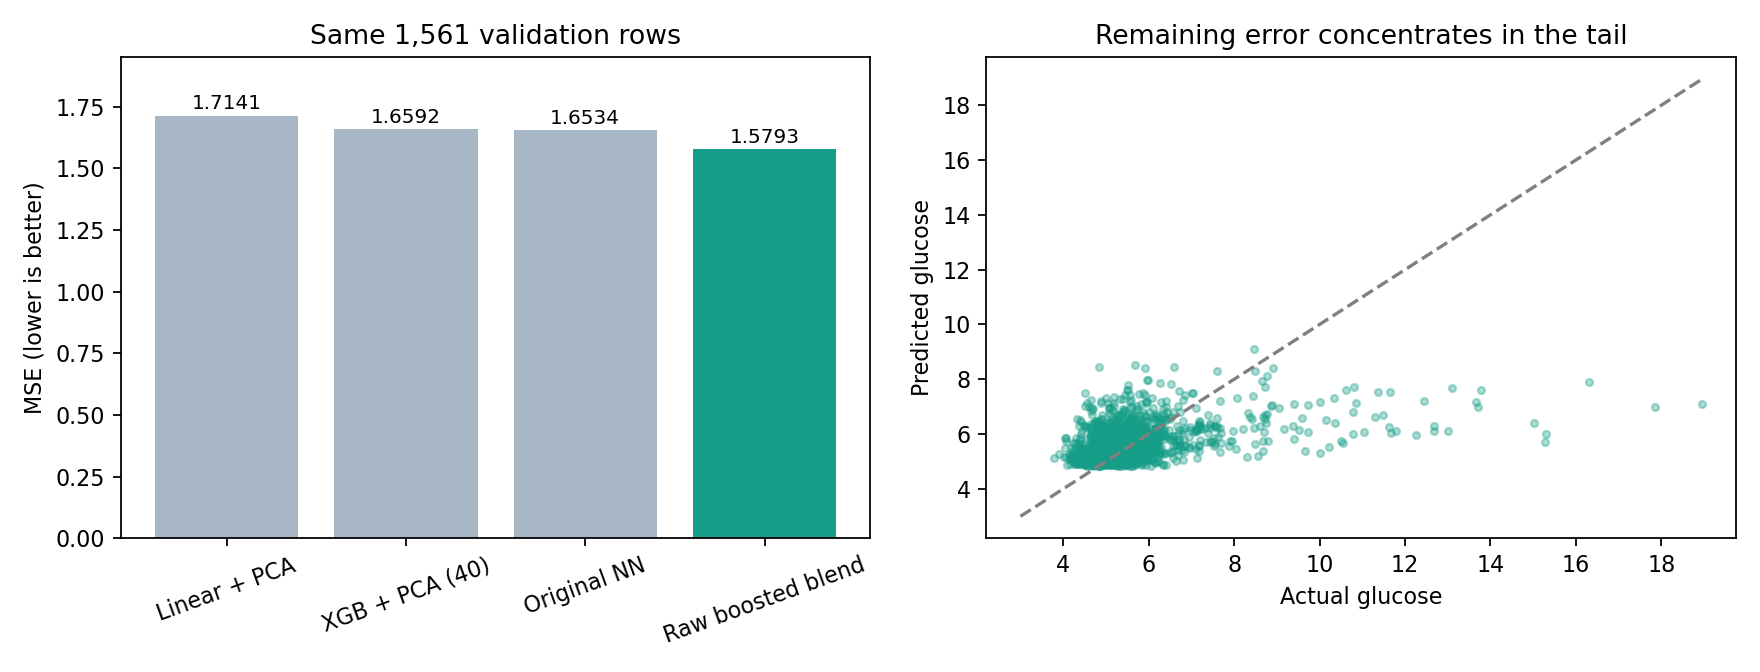
\includegraphics[width=0.94\linewidth,height=0.68\textheight,keepaspectratio]{paper/figures/paper_optimized_C004_O03.png}
\caption{历史H1的1561条验证记录对照；旧网络仅有历史汇总值，不能作为当前主协议成绩或配对推断依据。}
\label{fig:history}
\end{figure}

\section{完整预处理结果与探索图}\label{app:diagnostics}
表\ref{tab:holdout-all}给出42配置在开发/B的84行指标，均为固定配置的已知集合评价，不以其中最低B分数重新选型。自动缺失指示及PCA维数取决于拟合部分，420个折的维数与误差保存在相应结果表中，不统一指定为探索中的29维。
\begingroup
\small
\renewcommand{\arraystretch}{1.08}
\setlength{\tabcolsep}{5pt}
\begin{longtable}{lrrrrrr}
\caption{固定模型所有处理在开发/B的完整指标}\label{tab:holdout-all}\\
\toprule
集合 & 模型 & 处理 & MSE & RMSE & MAE & $R^2$ \\
\midrule
\endfirsthead
\caption[]{固定模型所有处理在开发/B的完整指标（续）}\\
\toprule
集合 & 模型 & 处理 & MSE & RMSE & MAE & $R^2$ \\
\midrule
\endhead
开发 & Ridge & raw & 2.287914 & 1.512585 & 0.810238 & 0.165007 \\
开发 & Ridge & scale & 2.289115 & 1.512982 & 0.807902 & 0.164568 \\
开发 & Ridge & pca & 2.496243 & 1.579950 & 0.825501 & 0.088975 \\
开发 & Ridge & scale\_pca & 2.325464 & 1.524947 & 0.812558 & 0.151303 \\
开发 & 决策树 & raw & 2.595176 & 1.610955 & 0.829650 & 0.052869 \\
开发 & 决策树 & scale & 2.595176 & 1.610955 & 0.829650 & 0.052869 \\
开发 & 决策树 & pca & 2.593023 & 1.610287 & 0.832673 & 0.053655 \\
开发 & 决策树 & scale\_pca & 2.601778 & 1.613003 & 0.846984 & 0.050459 \\
开发 & AdaBoost & raw & 2.455500 & 1.567004 & 0.808051 & 0.103845 \\
开发 & AdaBoost & scale & 2.456175 & 1.567219 & 0.809142 & 0.103598 \\
开发 & AdaBoost & pca & 2.558242 & 1.599451 & 0.847043 & 0.066348 \\
开发 & AdaBoost & scale\_pca & 2.576916 & 1.605278 & 0.837201 & 0.059533 \\
开发 & 随机森林 & raw & 2.276036 & 1.508654 & 0.786652 & 0.169341 \\
开发 & 随机森林 & scale & 2.275386 & 1.508438 & 0.786612 & 0.169579 \\
开发 & 随机森林 & pca & 2.478859 & 1.574439 & 0.814068 & 0.095319 \\
开发 & 随机森林 & scale\_pca & 2.380177 & 1.542782 & 0.804430 & 0.131334 \\
开发 & 原XGB & raw & 2.228808 & 1.492919 & 0.780951 & 0.186578 \\
开发 & 原XGB & scale & 2.228808 & 1.492919 & 0.780951 & 0.186578 \\
开发 & 原XGB & pca & 2.461235 & 1.568832 & 0.804223 & 0.101752 \\
开发 & 原XGB & scale\_pca & 2.337533 & 1.528899 & 0.804432 & 0.146898 \\
开发 & 优化XGB & raw & 2.236749 & 1.495577 & 0.782494 & 0.183680 \\
开发 & 优化XGB & scale & 2.236749 & 1.495577 & 0.782494 & 0.183680 \\
开发 & 优化XGB & pca & 2.606732 & 1.614538 & 0.841462 & 0.048651 \\
开发 & 优化XGB & scale\_pca & 2.315206 & 1.521580 & 0.799018 & 0.155046 \\
开发 & LightGBM & raw & 2.191367 & 1.480327 & 0.788751 & 0.200242 \\
开发 & LightGBM & scale & 2.191424 & 1.480346 & 0.791429 & 0.200221 \\
开发 & LightGBM & pca & 2.667651 & 1.633295 & 0.854779 & 0.026418 \\
开发 & LightGBM & scale\_pca & 2.365943 & 1.538162 & 0.816030 & 0.136529 \\
开发 & LightGBM & native & 2.211554 & 1.487129 & 0.795697 & 0.192875 \\
开发 & HistGB & raw & 2.230219 & 1.493392 & 0.785259 & 0.186063 \\
开发 & HistGB & scale & 2.233692 & 1.494554 & 0.786407 & 0.184795 \\
开发 & HistGB & pca & 2.584429 & 1.607616 & 0.839956 & 0.056791 \\
开发 & HistGB & scale\_pca & 2.285720 & 1.511860 & 0.793138 & 0.165807 \\
开发 & HistGB & native & 2.218320 & 1.489403 & 0.787738 & 0.190405 \\
开发 & 原大网络 & raw & 2.619349 & 1.618440 & 0.790811 & 0.044046 \\
开发 & 原大网络 & scale & 2.333565 & 1.527601 & 0.739419 & 0.148346 \\
开发 & 原大网络 & pca & 2.513425 & 1.585379 & 0.768613 & 0.082704 \\
开发 & 原大网络 & scale\_pca & 2.395645 & 1.547787 & 0.748050 & 0.125689 \\
开发 & 小网络 & raw & 2.883043 & 1.697953 & 0.872168 & -0.052191 \\
开发 & 小网络 & scale & 2.260269 & 1.503419 & 0.820975 & 0.175096 \\
开发 & 小网络 & pca & 3.608054 & 1.899488 & 1.138812 & -0.316790 \\
开发 & 小网络 & scale\_pca & 2.316041 & 1.521855 & 0.822817 & 0.154741 \\
B & Ridge & raw & 1.375474 & 1.172806 & 0.714380 & 0.104320 \\
B & Ridge & scale & 1.372016 & 1.171331 & 0.711438 & 0.106572 \\
B & Ridge & pca & 1.456986 & 1.207057 & 0.710259 & 0.051242 \\
B & Ridge & scale\_pca & 1.369370 & 1.170201 & 0.705186 & 0.108295 \\
B & 决策树 & raw & 1.401940 & 1.184036 & 0.680730 & 0.087086 \\
B & 决策树 & scale & 1.401940 & 1.184036 & 0.680730 & 0.087086 \\
B & 决策树 & pca & 1.517168 & 1.231734 & 0.709635 & 0.012052 \\
B & 决策树 & scale\_pca & 1.576842 & 1.255724 & 0.749767 & -0.026806 \\
B & AdaBoost & raw & 1.444966 & 1.202067 & 0.709821 & 0.059069 \\
B & AdaBoost & scale & 1.446088 & 1.202534 & 0.708552 & 0.058338 \\
B & AdaBoost & pca & 1.508366 & 1.228155 & 0.745288 & 0.017784 \\
B & AdaBoost & scale\_pca & 1.510745 & 1.229124 & 0.748463 & 0.016235 \\
B & 随机森林 & raw & 1.334292 & 1.155116 & 0.664520 & 0.131137 \\
B & 随机森林 & scale & 1.332931 & 1.154526 & 0.663986 & 0.132023 \\
B & 随机森林 & pca & 1.477213 & 1.215407 & 0.700992 & 0.038070 \\
B & 随机森林 & scale\_pca & 1.446742 & 1.202806 & 0.707142 & 0.057912 \\
B & 原XGB & raw & 1.252744 & 1.119260 & 0.648007 & 0.184240 \\
B & 原XGB & scale & 1.252744 & 1.119260 & 0.648007 & 0.184240 \\
B & 原XGB & pca & 1.459217 & 1.207981 & 0.691446 & 0.049789 \\
B & 原XGB & scale\_pca & 1.367040 & 1.169205 & 0.681433 & 0.109813 \\
B & 优化XGB & raw & 1.242601 & 1.114720 & 0.646290 & 0.190845 \\
B & 优化XGB & scale & 1.242601 & 1.114720 & 0.646290 & 0.190845 \\
B & 优化XGB & pca & 1.512826 & 1.229970 & 0.696555 & 0.014880 \\
B & 优化XGB & scale\_pca & 1.305805 & 1.142718 & 0.674523 & 0.149688 \\
B & LightGBM & raw & 1.263230 & 1.123935 & 0.655432 & 0.177411 \\
B & LightGBM & scale & 1.253797 & 1.119731 & 0.660581 & 0.183554 \\
B & LightGBM & pca & 1.630577 & 1.276941 & 0.728529 & -0.061797 \\
B & LightGBM & scale\_pca & 1.386715 & 1.177589 & 0.677011 & 0.097001 \\
B & LightGBM & native & 1.268888 & 1.126449 & 0.652933 & 0.173727 \\
B & HistGB & raw & 1.257199 & 1.121249 & 0.659121 & 0.181339 \\
B & HistGB & scale & 1.257199 & 1.121249 & 0.659120 & 0.181338 \\
B & HistGB & pca & 1.517058 & 1.231689 & 0.703089 & 0.012124 \\
B & HistGB & scale\_pca & 1.353061 & 1.163212 & 0.695379 & 0.118915 \\
B & HistGB & native & 1.265633 & 1.125004 & 0.657481 & 0.175846 \\
B & 原大网络 & raw & 1.380860 & 1.175100 & 0.648097 & 0.100814 \\
B & 原大网络 & scale & 1.299368 & 1.139898 & 0.588549 & 0.153879 \\
B & 原大网络 & pca & 1.394061 & 1.180704 & 0.627414 & 0.092217 \\
B & 原大网络 & scale\_pca & 1.334516 & 1.155213 & 0.593131 & 0.130991 \\
B & 小网络 & raw & 1.451214 & 1.204663 & 0.629196 & 0.055000 \\
B & 小网络 & scale & 1.352561 & 1.162997 & 0.668018 & 0.119241 \\
B & 小网络 & pca & 1.764104 & 1.328196 & 0.793369 & -0.148747 \\
B & 小网络 & scale\_pca & 1.369101 & 1.170086 & 0.686410 & 0.108470 \\
\bottomrule
\end{longtable}
\endgroup

\clearpage

以下图除相关热图按原计算步骤重排外，均原样提取自保存Notebook。图\ref{fig:box1}和图\ref{fig:box2}使用填补后的训练副本且混合量纲，不能据其绝对高度跨变量比较离散程度。图\ref{fig:ols-residual}和图\ref{fig:ols-qq}仅反映OLS训练拟合；图\ref{fig:correlation}仅含输入，省略过密的格内数值，完整相关矩阵随稿提供。图\ref{fig:pca-diagnostic}只描述探索输入方差。图\ref{fig:nn-inner}反映原大网络内部选择，不是开发或B的学习曲线。
\begin{figure}[htbp]
\centering
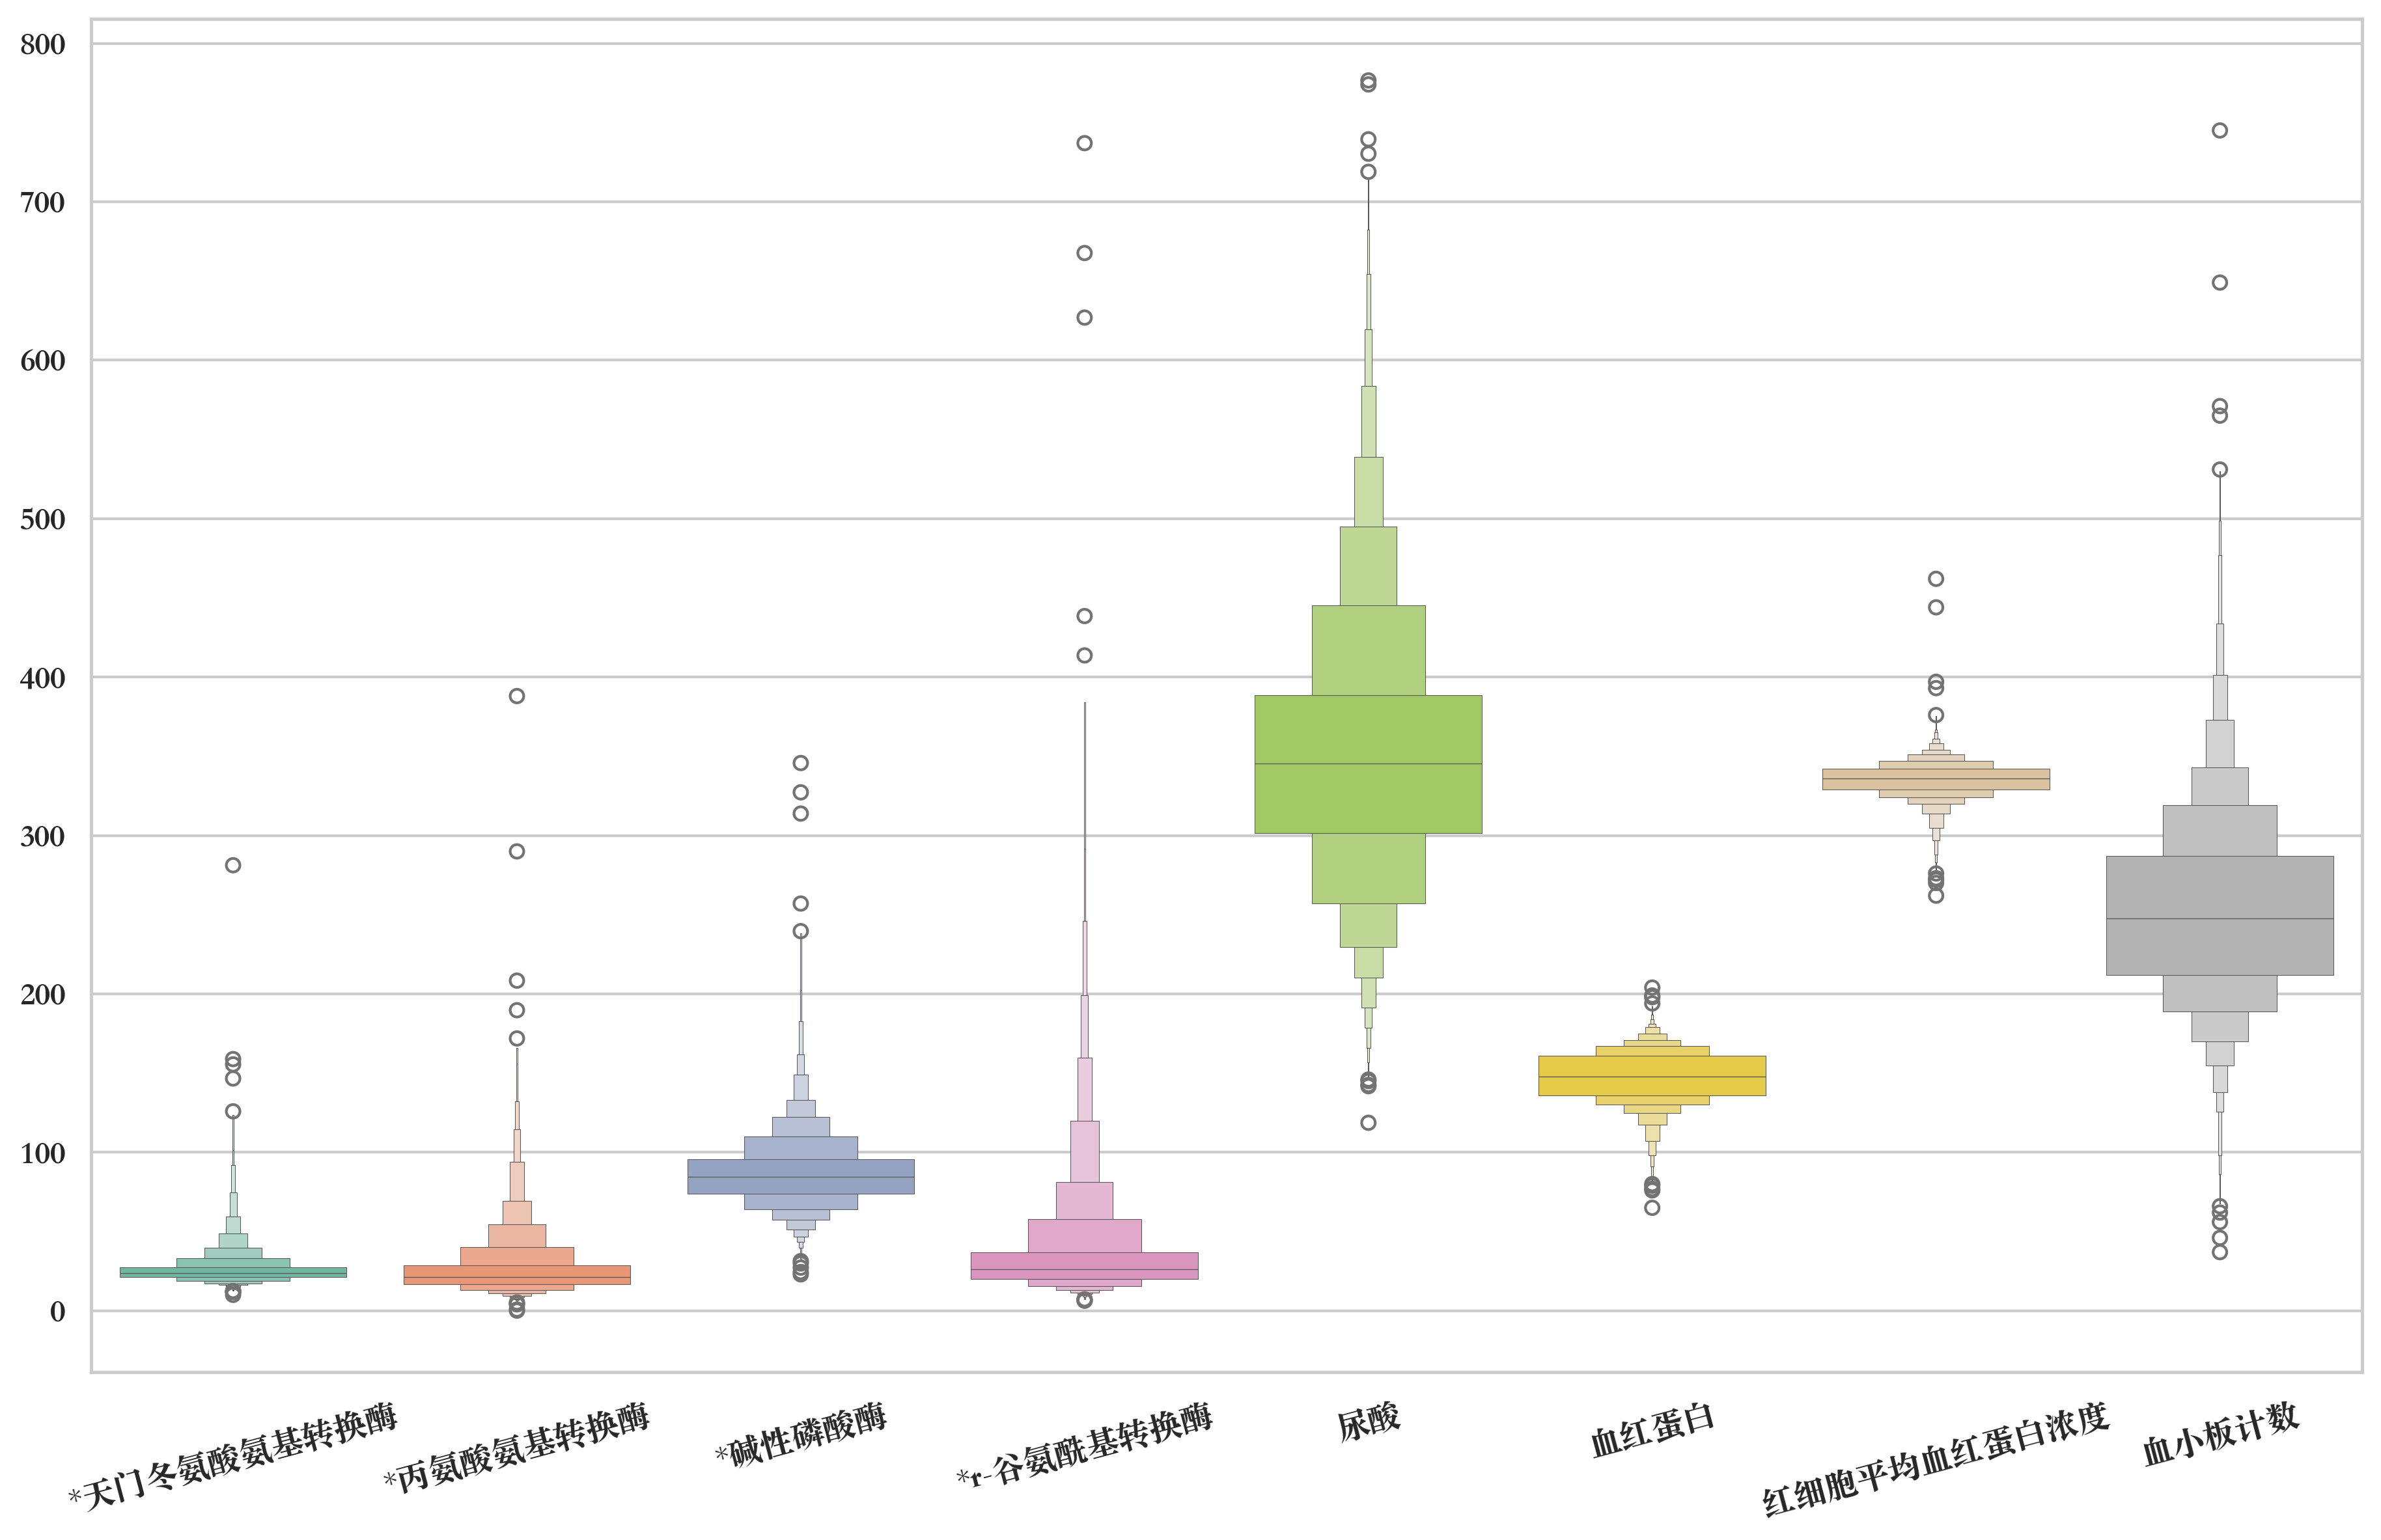
\includegraphics[width=0.94\linewidth,height=0.68\textheight,keepaspectratio]{paper/figures/paper_C026_O01.png}
\caption{训练填补副本的部分指标boxen图；指标量纲不同，图中极端记录均保留。}
\label{fig:box1}
\end{figure}
\begin{figure}[htbp]
\centering
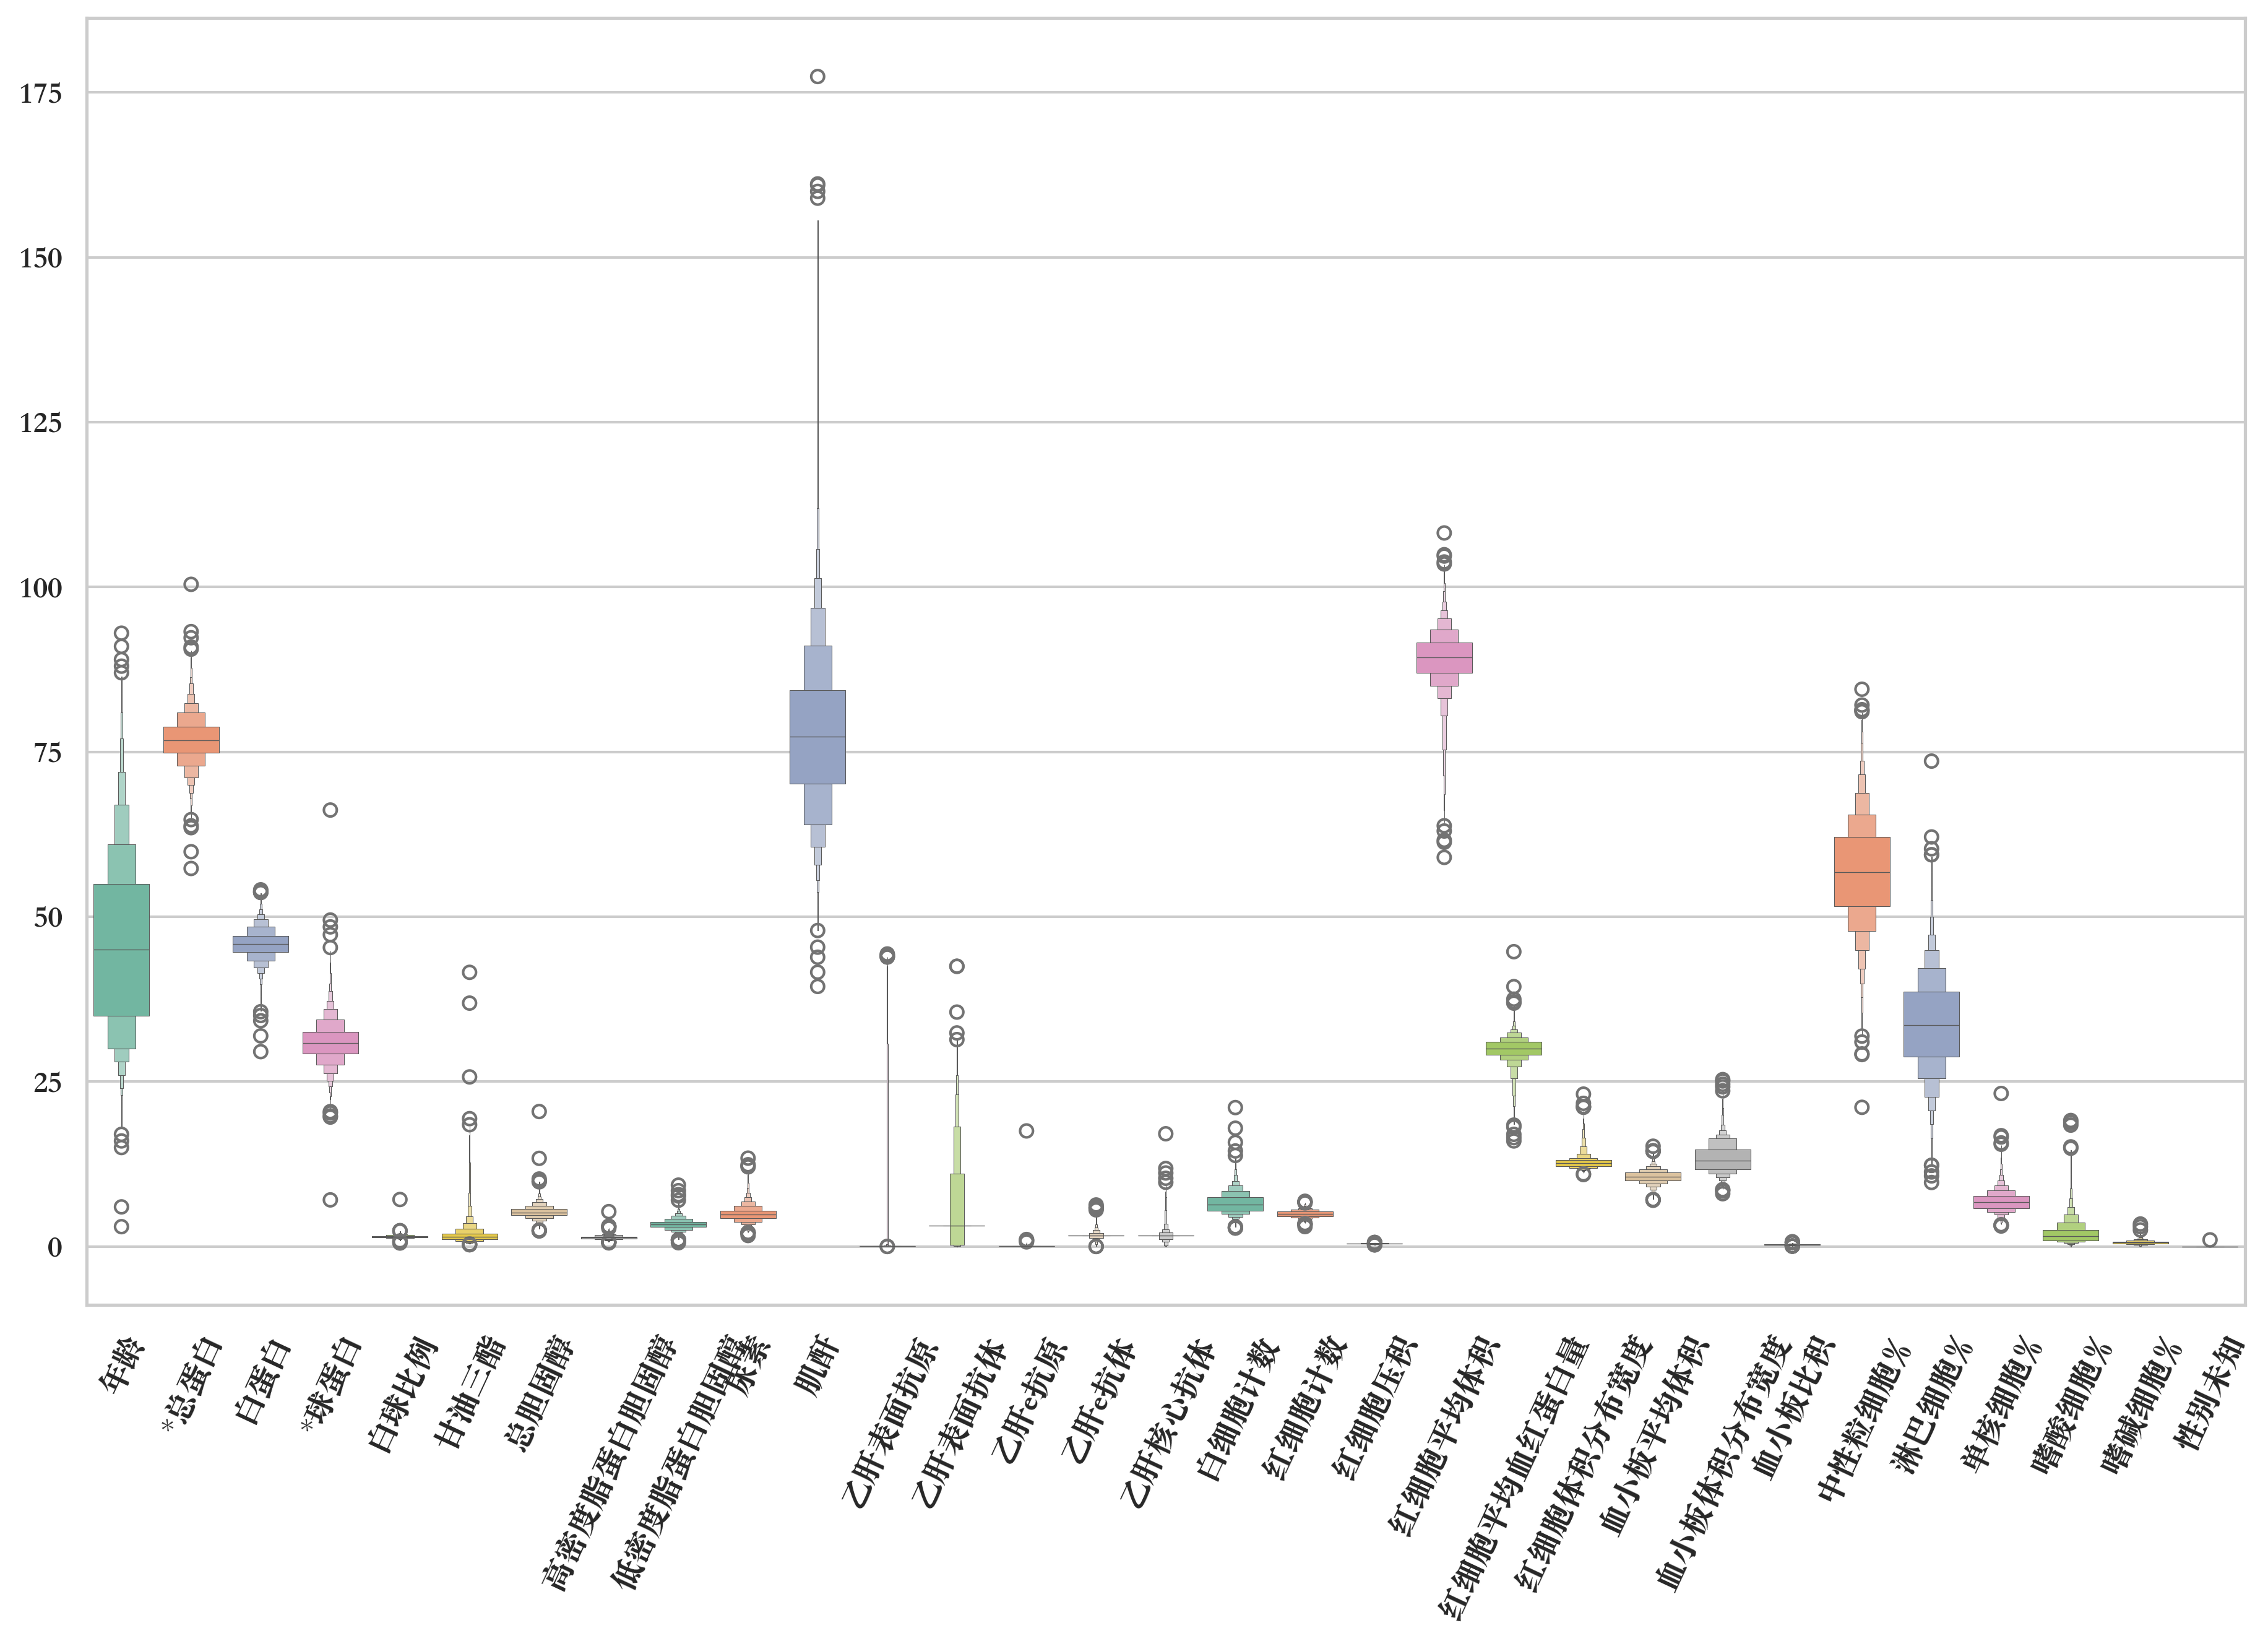
\includegraphics[width=0.94\linewidth,height=0.68\textheight,keepaspectratio]{paper/figures/paper_C027_O01.png}
\caption{训练填补副本的其余输入boxen图，包含年龄及未知指示等不同尺度变量。}
\label{fig:box2}
\end{figure}
\begin{figure}[htbp]
\centering
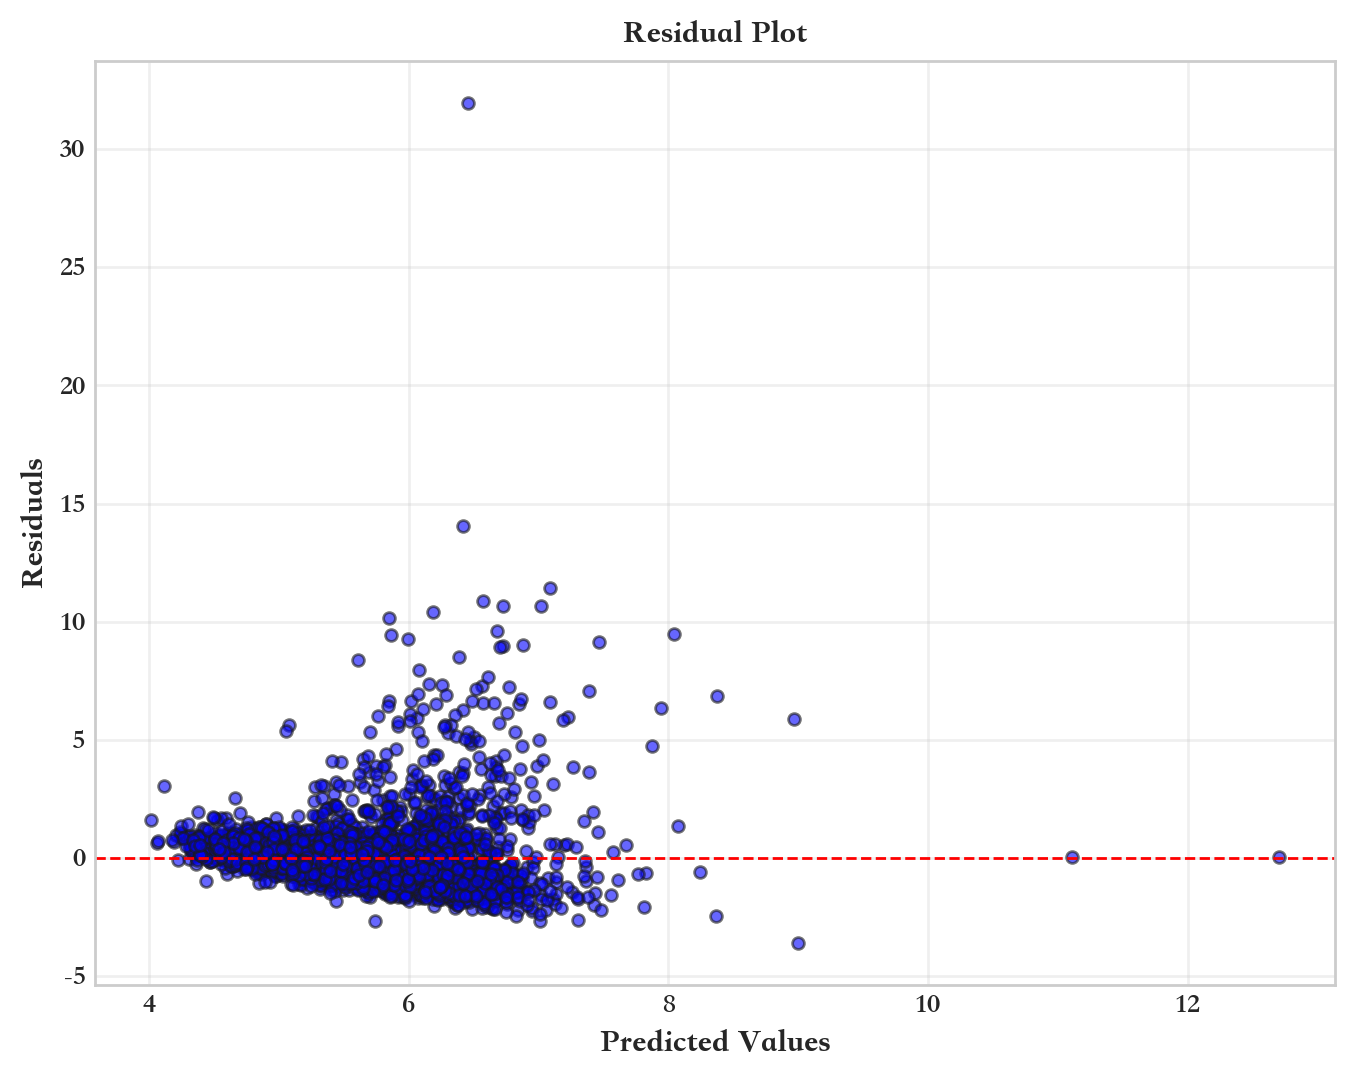
\includegraphics[width=0.94\linewidth,height=0.68\textheight,keepaspectratio]{paper/figures/paper_C032_O02.png}
\caption{OLS训练拟合残差图，不是最终融合开发或B集残差。}
\label{fig:ols-residual}
\end{figure}
\begin{figure}[htbp]
\centering
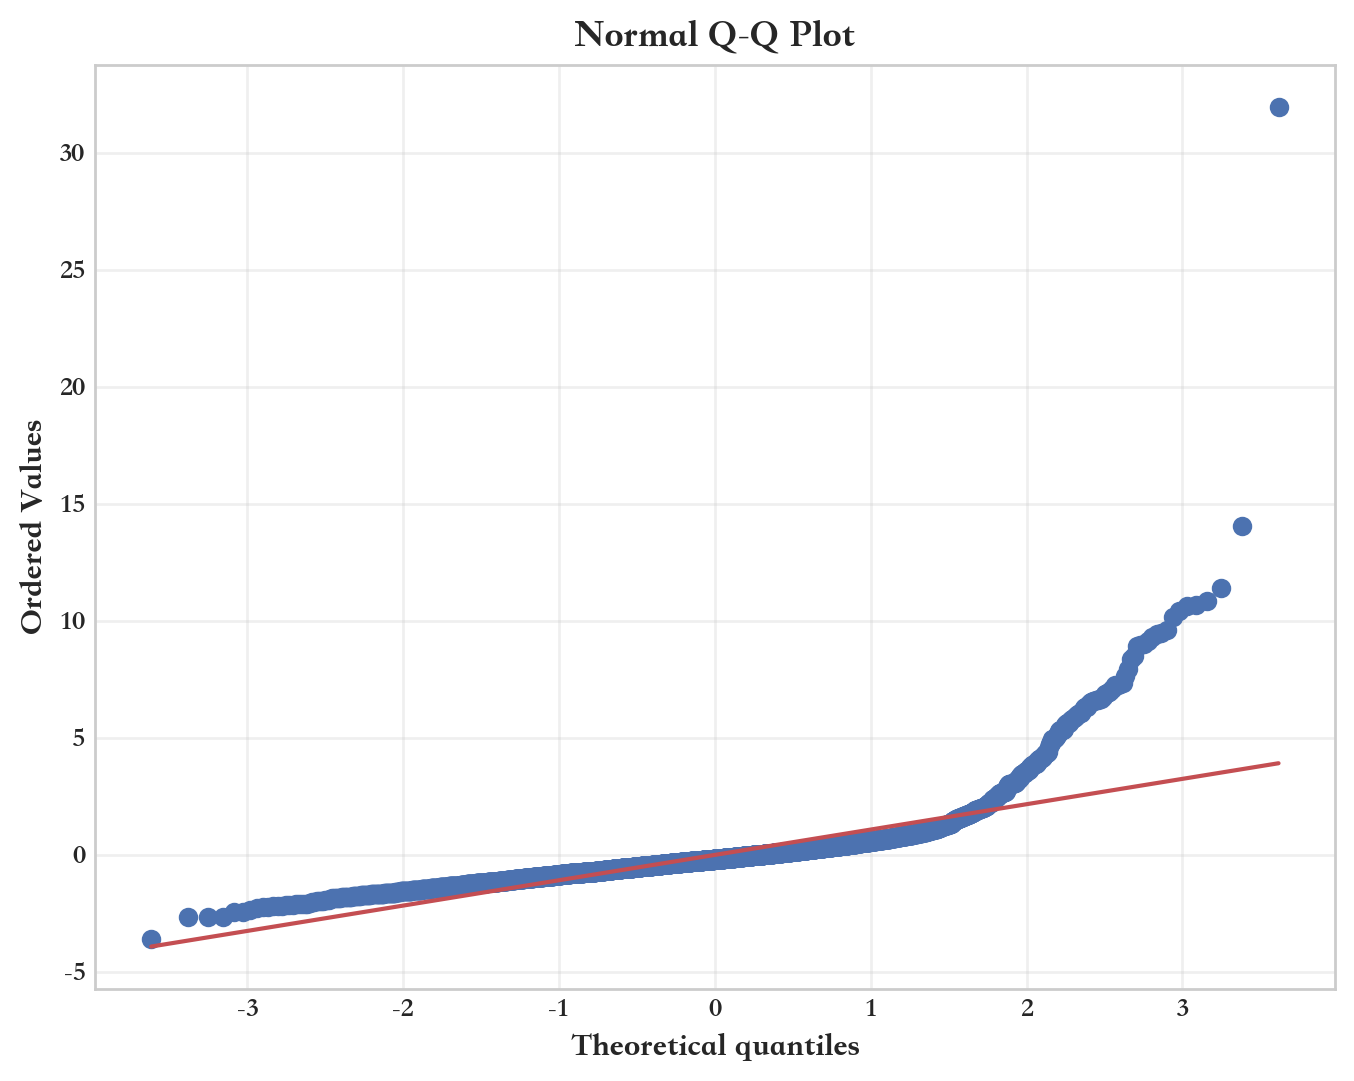
\includegraphics[width=0.94\linewidth,height=0.68\textheight,keepaspectratio]{paper/figures/paper_C032_O03.png}
\caption{OLS训练残差Q--Q图。}
\label{fig:ols-qq}
\end{figure}
\begin{figure}[p]
\centering
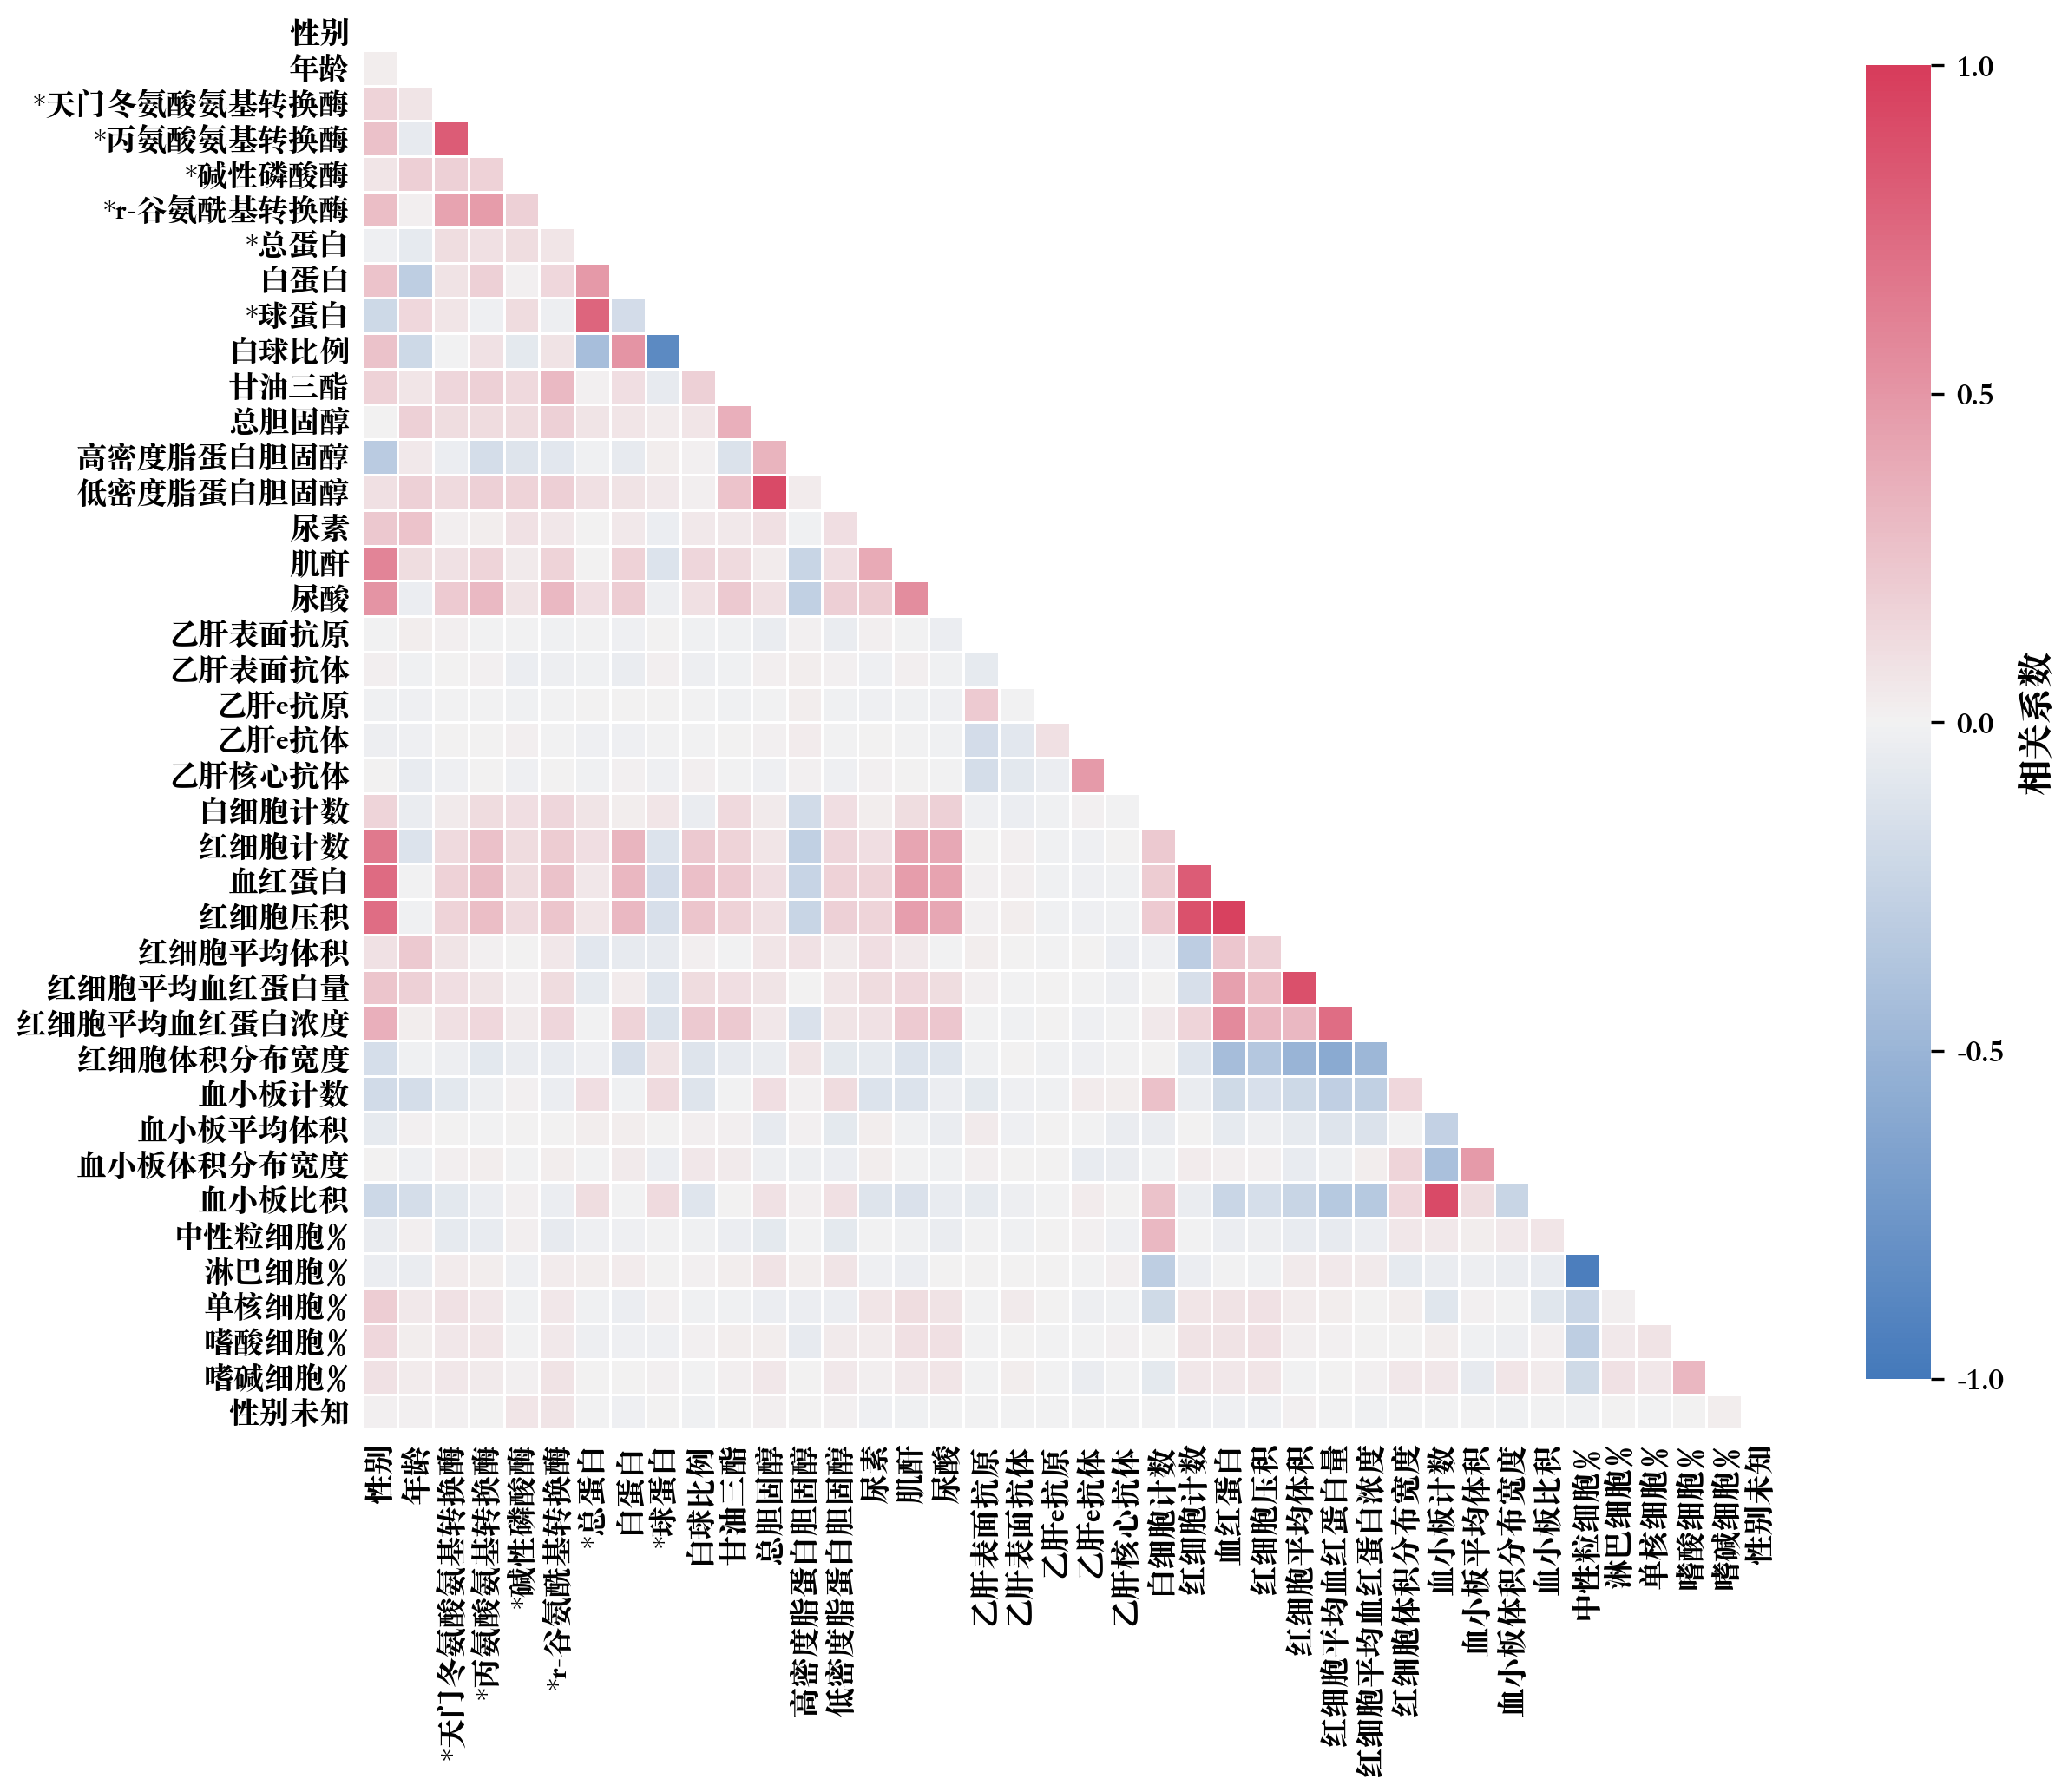
\includegraphics[width=0.94\linewidth,height=0.82\textheight,keepaspectratio]{paper/figures/training_correlation_reformatted.png}
\caption{40列训练探索输入相关热图，按原训练行与变换步骤重排；不包含血糖目标，填补及成组缺失可能影响相关结构。}
\label{fig:correlation}
\end{figure}
\begin{figure}[htbp]
\centering
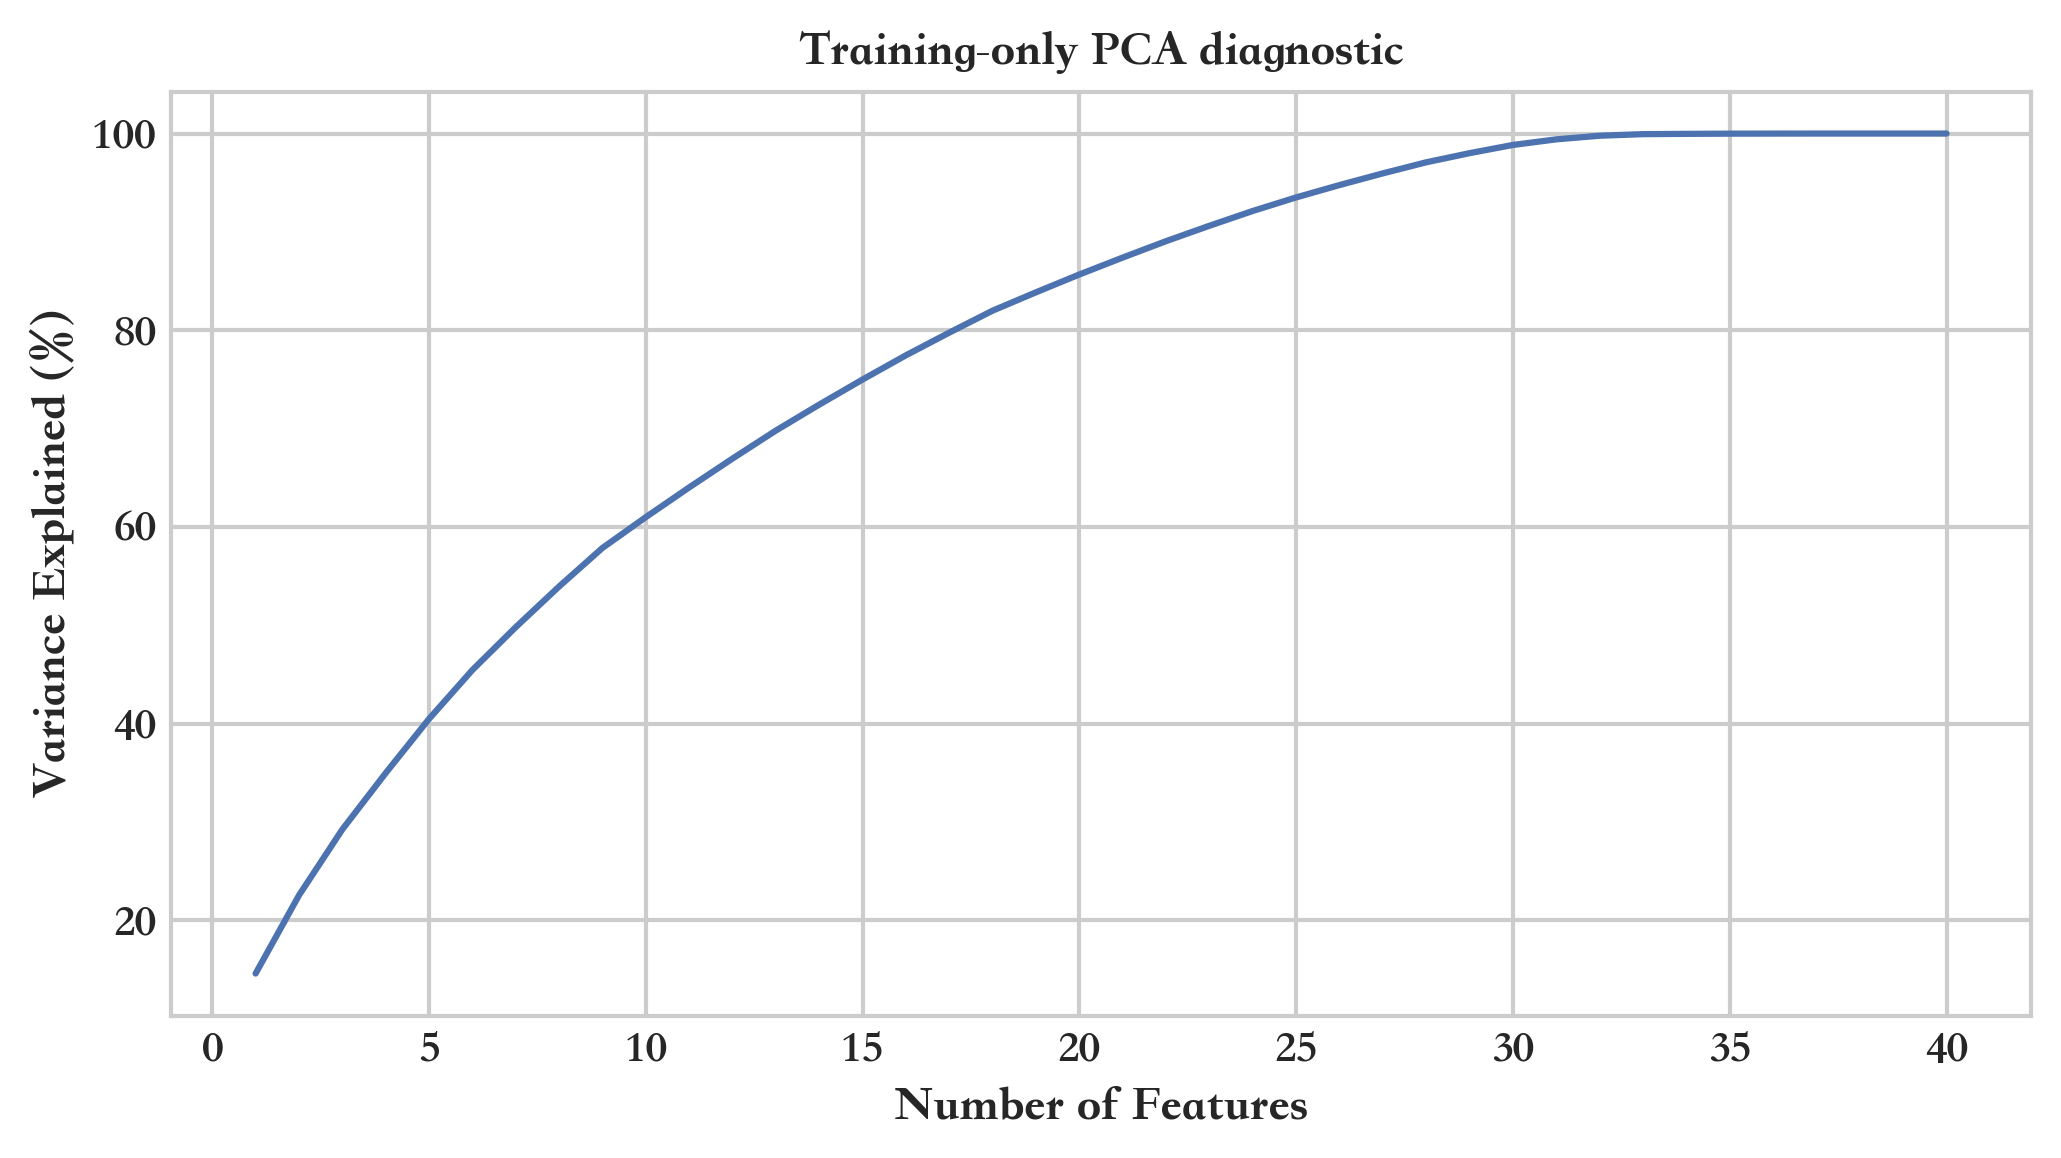
\includegraphics[width=0.94\linewidth,height=0.68\textheight,keepaspectratio]{paper/figures/paper_C040_O02.png}
\caption{训练探索矩阵的PCA累计方差；原图横轴应理解为成分序号，不是各预测折统一输入维数。}
\label{fig:pca-diagnostic}
\end{figure}
\begin{figure}[htbp]
\centering
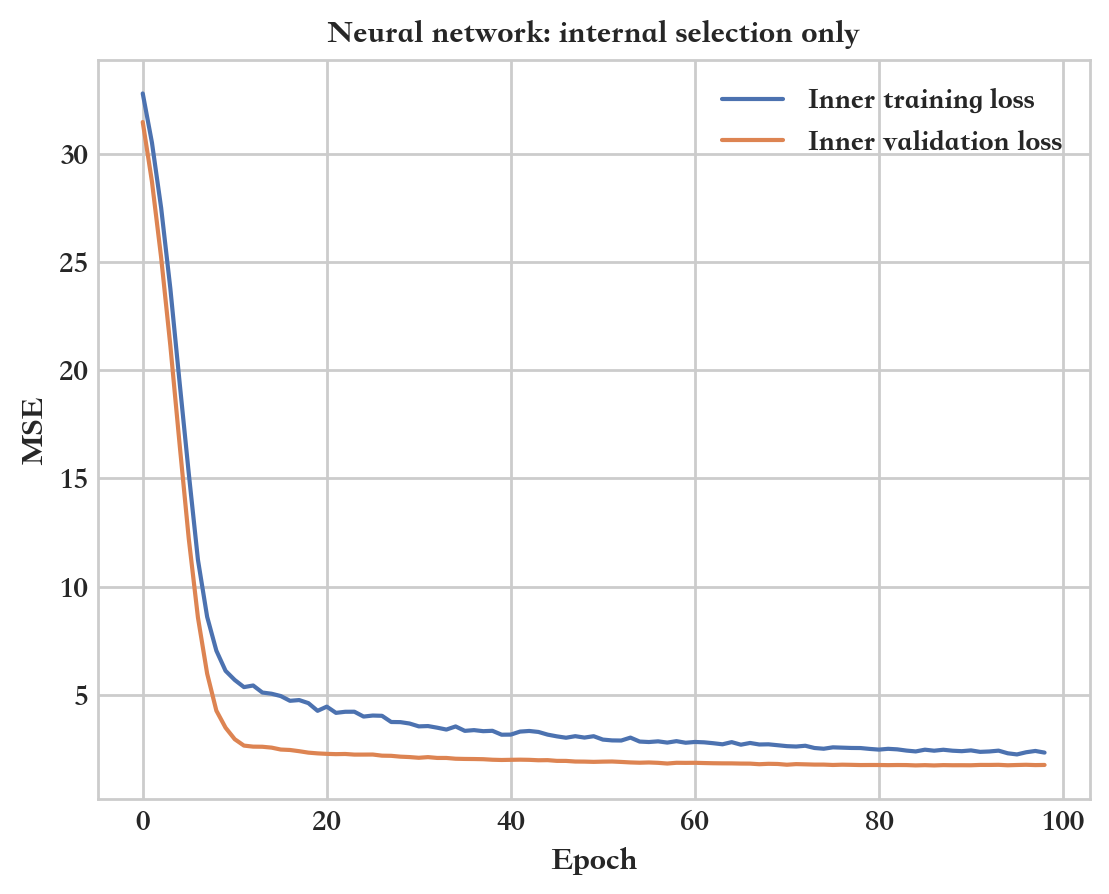
\includegraphics[width=0.94\linewidth,height=0.68\textheight,keepaspectratio]{paper/figures/paper_C051_O02.png}
\caption{原大网络内部表示与轮数选择的损失曲线；不是开发/B训练曲线。}
\label{fig:nn-inner}
\end{figure}

\section{研究来源与结果追溯}\label{app:provenance}
主Notebook提供数据、探索、六模型和后续结果入口，顺序及预处理Notebook主要展示已完成的实验产物，训练实现在对应执行脚本。Notebook单元格统一按cells数组从1计数，记C001等，不用可能重新开始的执行计数作唯一标识。
表\ref{tab:provenance}给出主要研究环节的来源位置。
\begin{table}[htbp]
\footnotesize
\setlength{\tabcolsep}{5pt}
\centering
\caption{研究环节的Notebook与文件定位}
\label{tab:provenance}
\begin{tabular}{L{0.2\linewidth}L{0.24\linewidth}L{0.46\linewidth}}
\toprule
研究内容 & Notebook定位 & 存档/实现定位 \\
\midrule
数据与训练探索 & 主C002/C005--C044 & 原始CSV、数据划分id与探索输出 \\
原六模型 & 主C046--C071 & external\_b\_comparison冻结配置、comparison及predictions \\
特征/联合搜索 & 顺序C004/C006 & run\_experiments及feature\_ablation/training\_cv \\
网络补充/融合 & 顺序C008--C012 & refine\_nn\_features、complete\_nn\_blends及冻结选择 \\
主结果及区间 & 顺序C014；主C072 & evaluation、paired\_intervals、target\_bands及逐行预测 \\
预处理对照 & 预处理C004--C014；主C073 & run\_ablation、frozen\_recommendations与holdout指标 \\
历史协议 & 早期C004--C010 & paper\_optimized及optimization两协议结果 \\
\bottomrule
\end{tabular}
\end{table}


正文主要公式、数值、图表与上述来源的逐项关系另列于随稿来源核对表。原有独立指标复核包含1090项保存值与预测计算的比较，绝对容差$5\times10^{-7}$内一致，最大差约$2.0522\times10^{-8}$；该数量包含同源指标，不是独立实验次数。原始六模型开发结果中，大网络等部分以保存输出追溯，不能将所有开发指标都说成已由完整逐条预测存档独立重算。已有模型重载核验是历史运行证据，本文整理过程未重训或重新开展模型实验。

\clearpage
\end{document}
